% Dieser Text ist urheberrechtlich gesch\"utzt
% Er stellt einen Auszug eines von mir erstellten Referates da
% und darf nicht gewerblich genutzt werden
% die private bzw. Studiums bezogen Nutzung ist frei
% April 2011
% Autor: Sascha Frank 
% Universit\"at Freiburg 
% www.informatik.uni-freiburg.de/~frank/
% frank < was da sonst immer steht > tf.uni-freiburg.de
\documentclass[hyperref={pdfpagelabels=false}]{beamer}
% Die Hyperref Option hyperref={pdfpagelabels=false} verhindert die Warnung:
% Package hyperref Warning: Option `pdfpagelabels' is turned off
% (hyperref)                because \thepage is undefined. 
% Hyperref stopped early 
\usetheme{Warsaw}
\beamertemplatenavigationsymbolsempty
\usepackage[T1]{fontenc}
%\usepackage[ngerman]{babel}
\usepackage[utf8]{inputenc}
\usepackage{amsmath,amsfonts,amssymb}
\usepackage{multimedia}
\usepackage{textcomp}
\usepackage{multirow}
\usepackage[sf,SF]{subfigure}
\usepackage{caption}
\usepackage{booktabs}
\usepackage{threeparttable}
\captionsetup[figure]{labelformat=empty}% redefines the caption setup of the figures environment in the beamer class.
\captionsetup[table]{labelformat=empty}% redefines the caption setup of the table environment in the beamer class.
\usepackage{upgreek}
\usepackage{lmodern}
% \usepackage{geometry}
% \usepackage[absolute,overlay]{textpos}
% Das Paket lmodern erspart die folgenden Warnungen:
% LaTeX Font Warning: Font shape `OT1/cmss/m/n' in size <4> not available
% (Font)              size <5> substituted on input line 22.
% LaTeX Font Warning: Size substitutions with differences
% (Font)              up to 1.0pt have occurred.
%
% Wenn \titel{\ldots} \author{\ldots} erst nach \begin{document} kommen,
% kommt folgende Warnung:
% Package hyperref Warning: Option `pdfauthor' has already been used,
% (hyperref) ... 
% Daher steht es hier vor \begin{document}
%\setbeamertemplate{headline}{} %%beseitigt Kopfzeile mit Kapitelübersicht und -navigation%%
%\setbeamertemplate{footline}{} %%beseitigt Fußzeile mit Namen und Titel%%
%\usepackage{biblatex}
%\bibliography{../Masterarbeit/Referenz}
\setbeamertemplate{footline}[frame number]
\setbeamerfont{frame number in foot}{size=\footnotesize}
% zusaetzlich ist das usepackage{beamerthemeshadow} eingebunden 
\usepackage{beamerthemeshadow}
% \beamersetuncovermixins{\opaqueness<1>{25}}{\opaqueness<2->{15}}
%  sorgt dafuer das die Elemente die erst noch (zukuenftig) kommen 
%  nur schwach angedeutet erscheinen 
% \beamersetuncovermixins{\opaqueness<1>{25}}{\opaqueness<2->{15}}
% klappt auch bei Tabellen, wenn teTeX verwendet wird\ldots
%\begin{document}

\begin{document}
\title{Water at $\upalpha$-Alumina Surfaces: Energetics, Dynamics and Kinetics}
\subtitle{{\bf Disputation}}   
\author{Sophia Heiden}
\institute{
\includegraphics[width=1.5cm]{figures/UP-Logo_Matjpg.jpg}}
% \date{\today} 
\date{xy.0z.2019}

\begin{frame}[plain]
 \addtocounter{framenumber}{-2}
\titlepage
\end{frame} 

\section[]{Introduction}
\begin{frame}[plain]
\frametitle{Outline}
 Investigation of Water on $\upalpha$-Alumina Surfaces: \newline 
\begin{itemize}
 \item \textbf{Motivation}
 \item \textbf{H$_2$O@$\upalpha$-Al$_2$O$_3$(0001)}: Stability, Vibrational Frequencies, and Reactivity
 \item \textbf{H$_2$O@$\upalpha$-Al$_2$O$_3$(0001)}: Molecular Beam Scattering with AIMD
 \item \textbf{H$_2$O@$\upalpha$-Al$_2$O$_3$(11\=20)}: Stability, Reactivity, and Vibrational Frequencies
 \item \textbf{Summary and Outlook}
 \end{itemize}
\end{frame}


\begin{frame}
 \frametitle{Motivation}
 \begin{columns}[c]
  \column{0.5\textwidth}
  \begin{itemize}
   \item Surface science, catalysis
   \item Computer based modelling of processes
  \end{itemize}
  \column{0.5\textwidth}
   \framebox{
   
\includegraphics[width=1.in]{figures/scientist-clipart-nerd.jpg}\tiny{$^1$} %https://mbtskoudsalg.com/images/scientist-clipart-nerd.jpg
   ~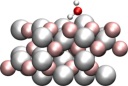
\includegraphics[width=1.in]{figures/surfaceprocess.pdf}}
 \end{columns}
 \pause
 \begin{columns}[c]
  \column{0.7\textwidth}
  Applications of Al$_2$O$_3$
  \begin{itemize}
   \item Ruby laser
   \item Catalyst: Claus process
   \item Ceramic material
   \item Solid rocket exhaust, eject alumina particles
  \end{itemize}
  \column{0.3\textwidth}
   \framebox{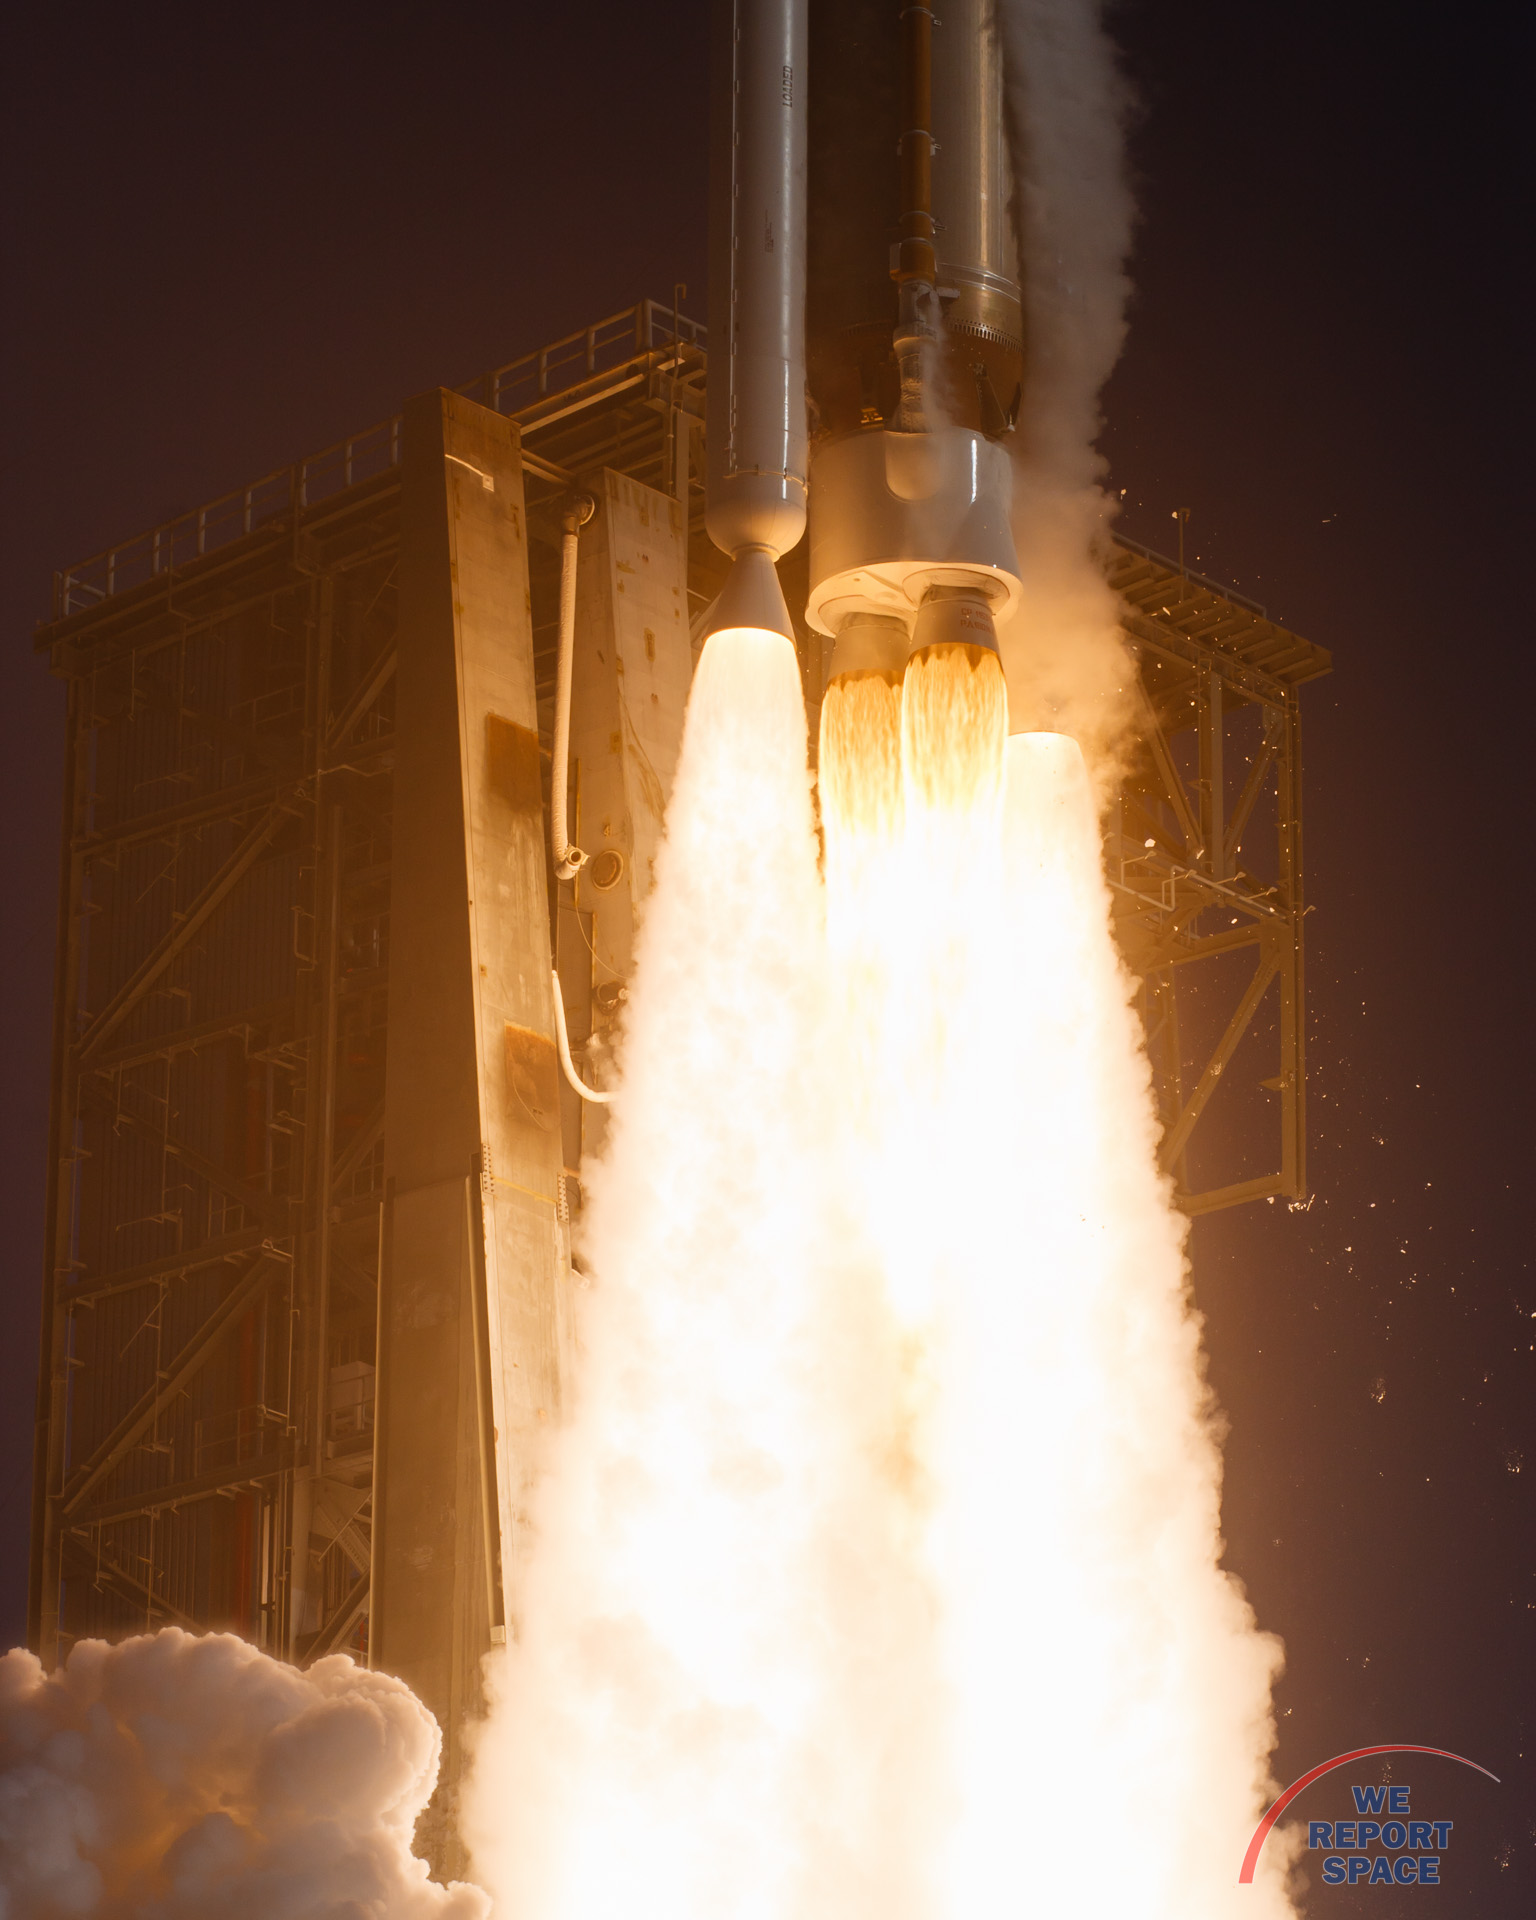
\includegraphics[width=1.in]{figures/8y0ObUW.jpg}}\tiny{$^2$} %https://external-preview.redd.it/raUdEwh8-J01prs80mqdLGG-sVTfg-80YXxwnfwVRtY.jpg?s=eabf5472b6d7a49b7a66ebfecade4f2b9d49dc2f
 \end{columns}
 ~\\
 \pause
 \boxed{\textbf{$\rightarrow$ Understanding processes on a microscopical scale!}}\\
 \tiny{$^1$ https://mbtskoudsalg.com/images/scientist-clipart-nerd.jpg, 
 $^2$https://external-preview.redd.it/raUdEwh8-J01prs80mqdLGG-sVTfg-80YXxwnfwVRtY.jpg?s=eabf5472b6d7a49b7a66ebfecade4f2b9d49dc2f}
\end{frame}


\begin{frame}
 \frametitle{Properties of $\upalpha$-Al$_2$O$_3$}
 \begin{columns}
  \column{.5\textwidth}
  \begin{figure}
  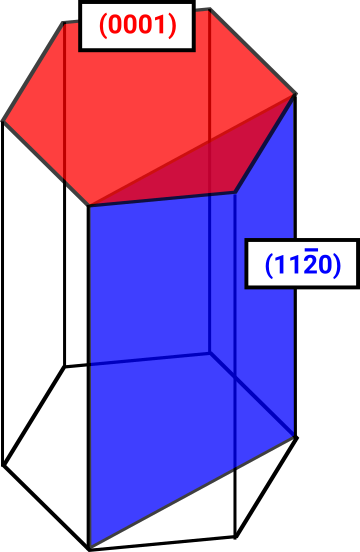
\includegraphics[width=0.3\textwidth]{figures/al2o3-crystal.png}
  \caption{Schematic view of the (0001) and (11\=20) surface cuts}
  \end{figure}
  \column{.5\textwidth}
  \begin{itemize}
  \item Hard
  \item Insulator
  \item Noncorrosive
  \item White solid, impurities can give color
  \item In UHV (0001) more stable than (11\=20)
  \end{itemize}
 \end{columns}
 \pause
\begin{columns}
  \column{.5\textwidth}
  \begin{figure}
  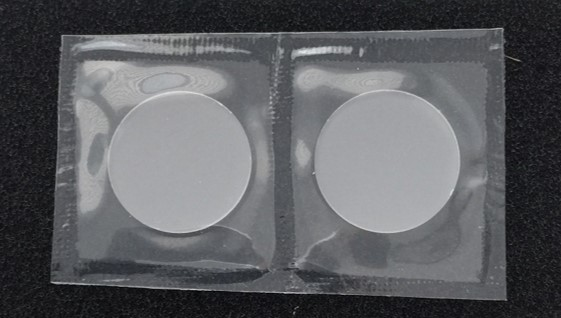
\includegraphics[width=0.6\textwidth]{figures/Al2O3.jpg}
  \caption{Alumina crystal used in experimental setup (FHI Berlin)}
 \end{figure}
  \column{.5\textwidth}
   \begin{figure}
  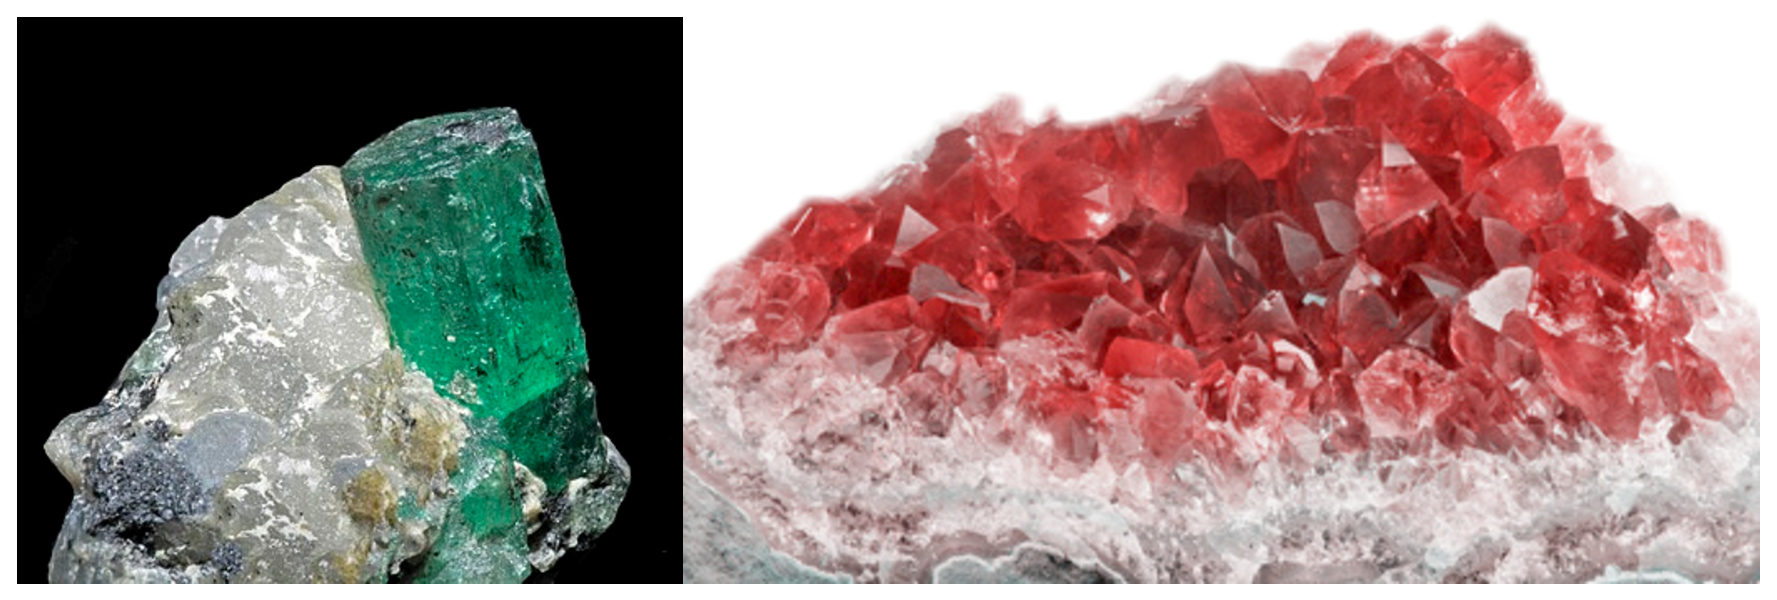
\includegraphics[width=0.6\textwidth]{figures/emerald-ruby.eps}
  \caption{Emerald (green, Cr/V); Ruby (red, Cr)}
  \end{figure}
 \end{columns}
\end{frame}

\begin{frame}
 \frametitle{Methodology}
 \begin{itemize}
  \item Electronic structure calculations (KS-DFT, HF, LMP2)
  \begin{equation*}
    \left(-\frac{1}{2}\vec{\nabla}^2_1 + v_{ext}(\vec{r}_1) + v_{H}(\vec{r}_1) + v_{xc}(\vec{r}_1) \right)\psi^{KS}_i(\vec{r}_1) = \varepsilon_i^{KS}\psi^{KS}_i(\vec{r}_1)
  \end{equation*}
  \pause
  \item Vibrational frequencies (harmonic approximation)
  \begin{equation*}
    \textbf{H} \vec{A}_i=\lambda_i\vec{A}_i; ~~~  \omega_i=\sqrt{\lambda_i}
  \end{equation*}
  \pause
  \item \textit{Ab-initio} molecular dynamics
    \begin{equation*}
      -\vec{\nabla}_A V(\{\vec{R}_i\})=M_A\frac{d^2 \vec{R}_A(t)}{dt^2}
    \end{equation*}
 \end{itemize}
\end{frame}


\begin{frame}
 \frametitle{Methodology}
 \begin{itemize}
  \item Periodic slab calculations
  \item Density functional theory
  \item GGA functional PBE with dispersion corrections in PW basis
  \item VASP program package
 \end{itemize}
 \begin{itemize}
  \item PBE, B3LYP with dispersion corrections and LMP2, in AO basis
  \item CRYSTAL and CRYSCOR
 \end{itemize}
 \centering
 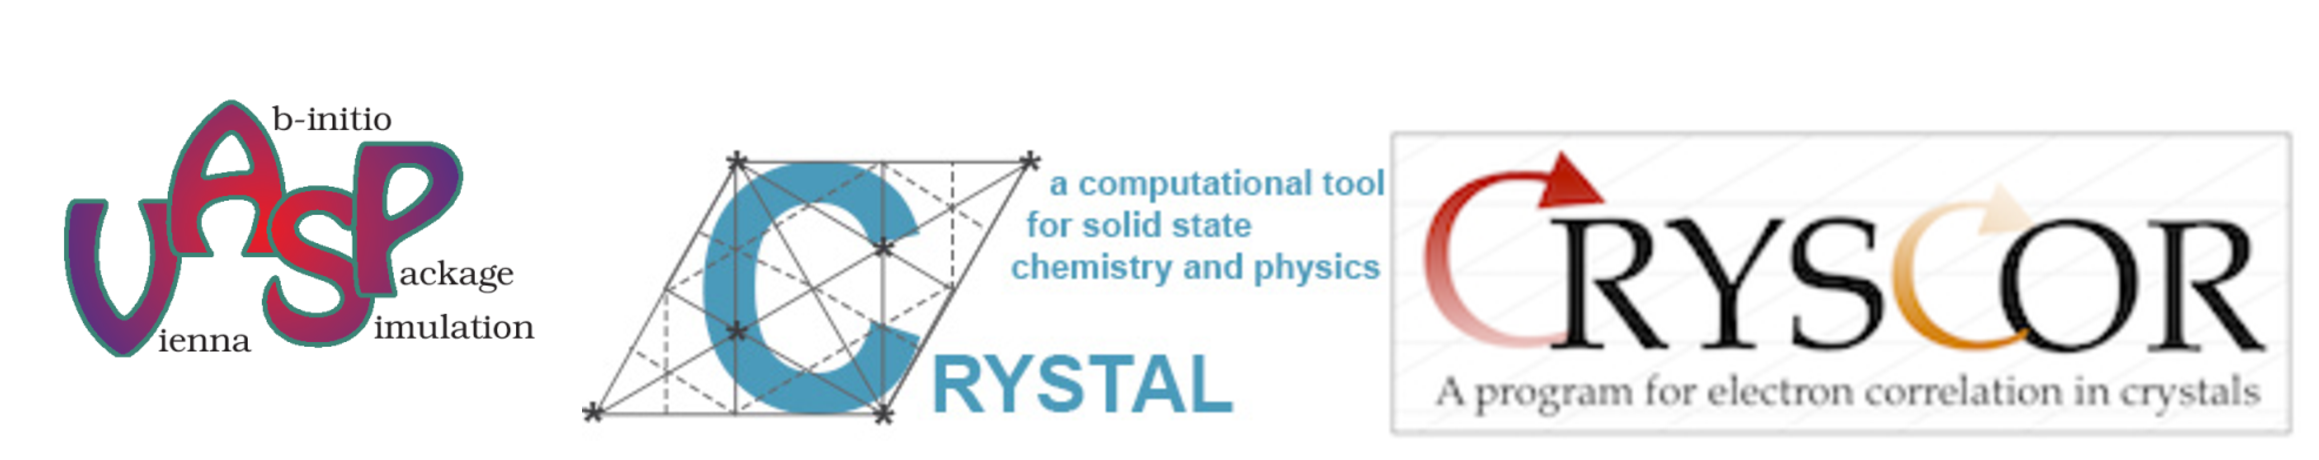
\includegraphics[width=0.7\textwidth]{figures/programs-logos.eps}
\end{frame}

\section{Water@$\upalpha$-Al$_2$O$_3$(0001): Stability, Vibrations, and Reactivity}
\begin{frame}
 \frametitle{Model of the Al$_2$O$_3$(0001) Surface}
 \begin{columns}
  \column{0.5\textwidth}
   \begin{figure}
  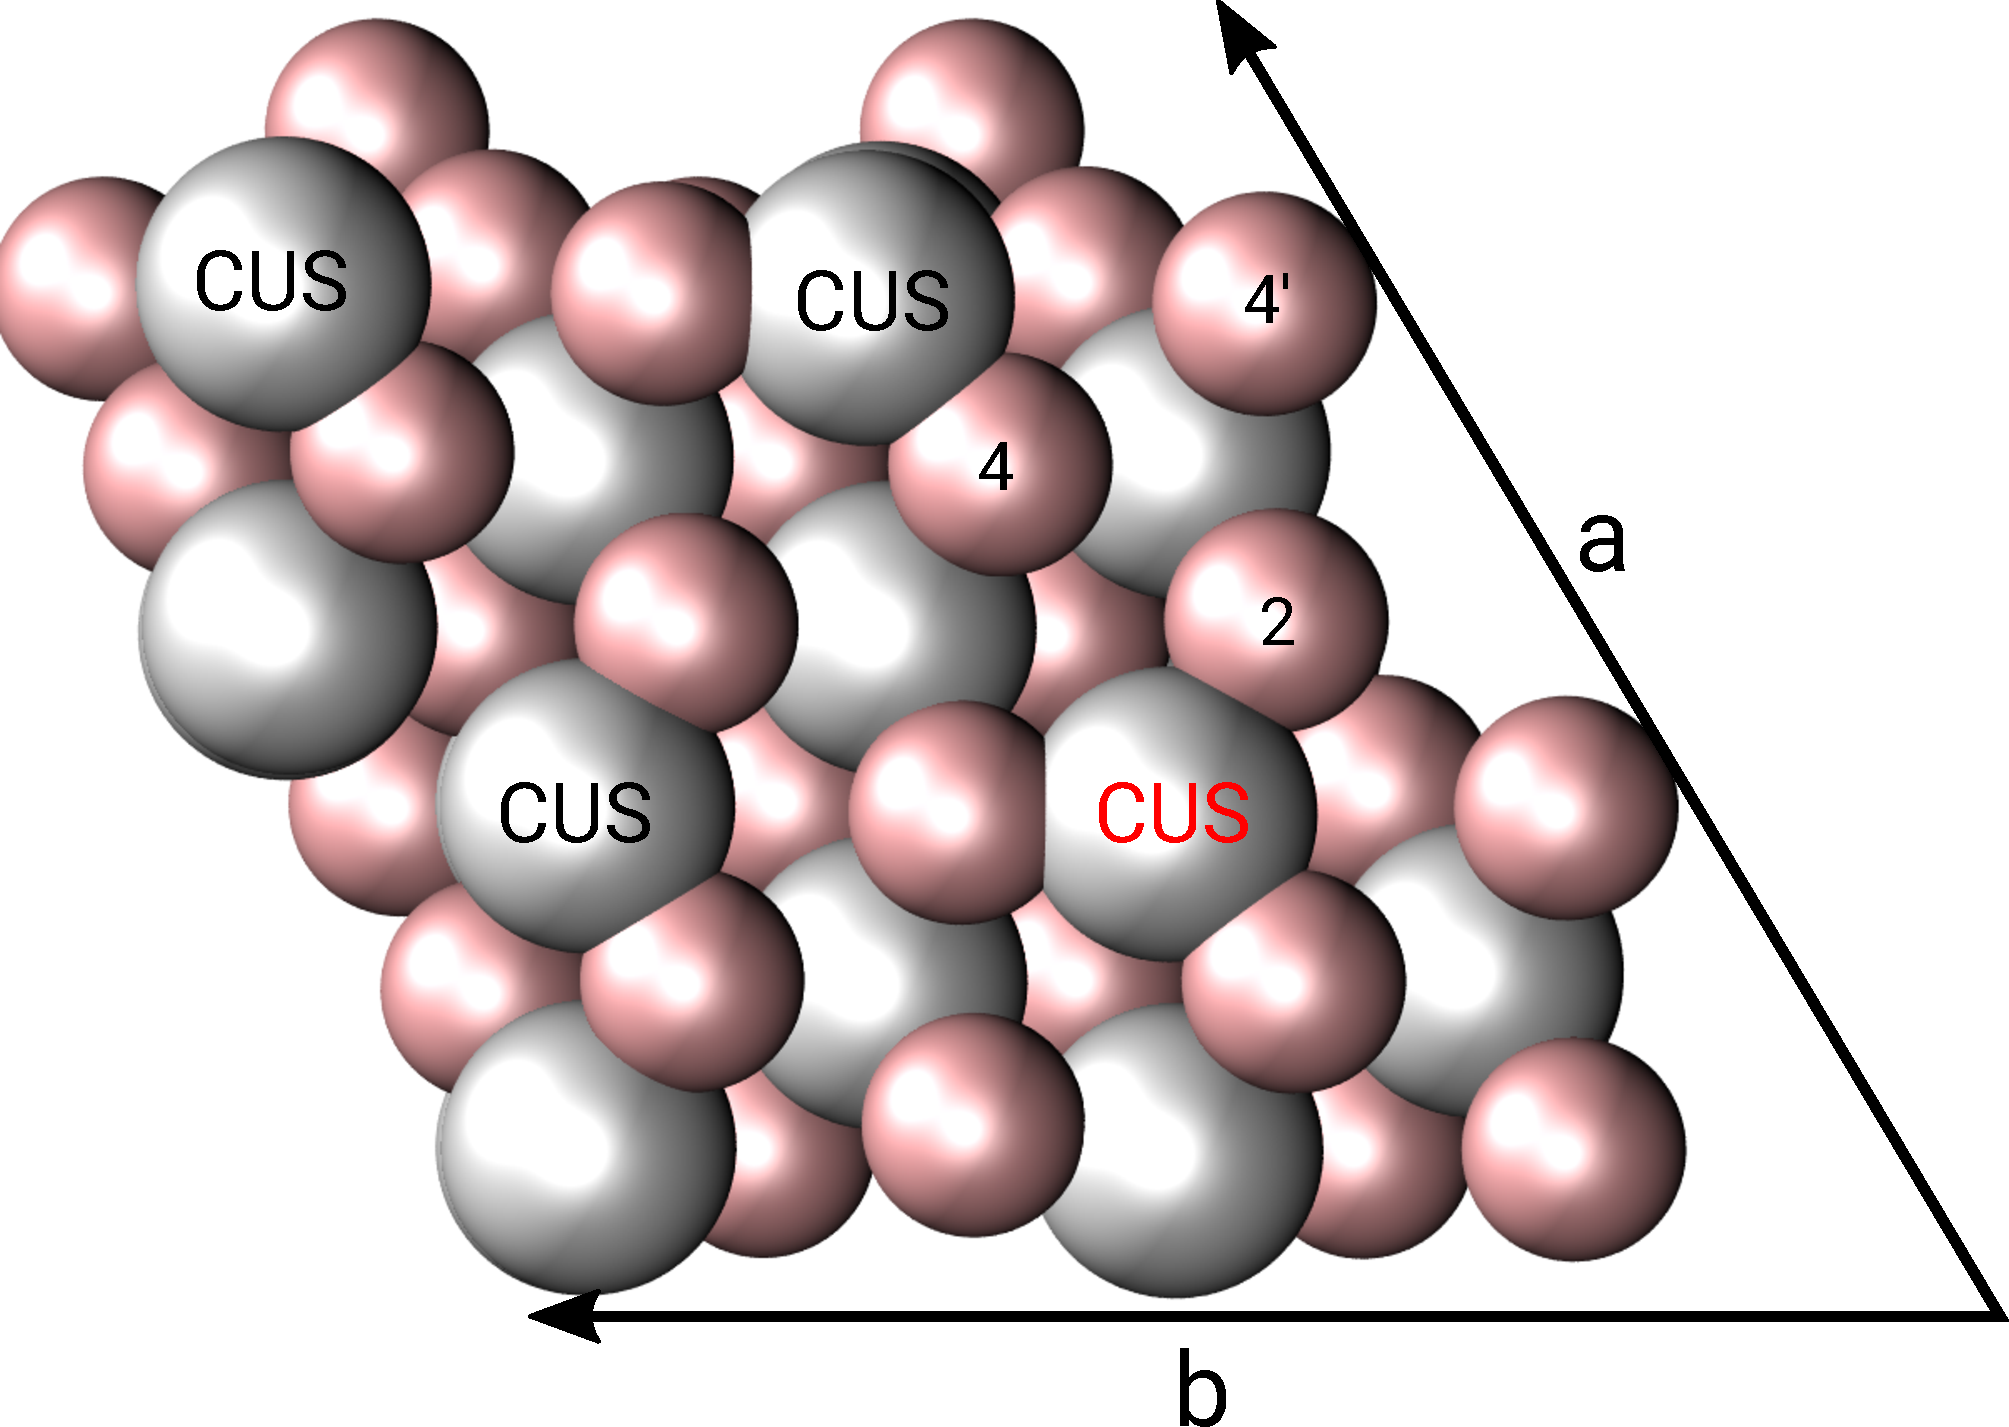
\includegraphics[width=0.9\textwidth]{figures/surf_0K_axes.pdf}
  \caption{Top view, Al gray, O pink. \textbf{C}oordinatively \textbf{U}nsaturated \textbf{S}ite}
  \end{figure}
  \column{0.5\textwidth}
  \begin{figure}
  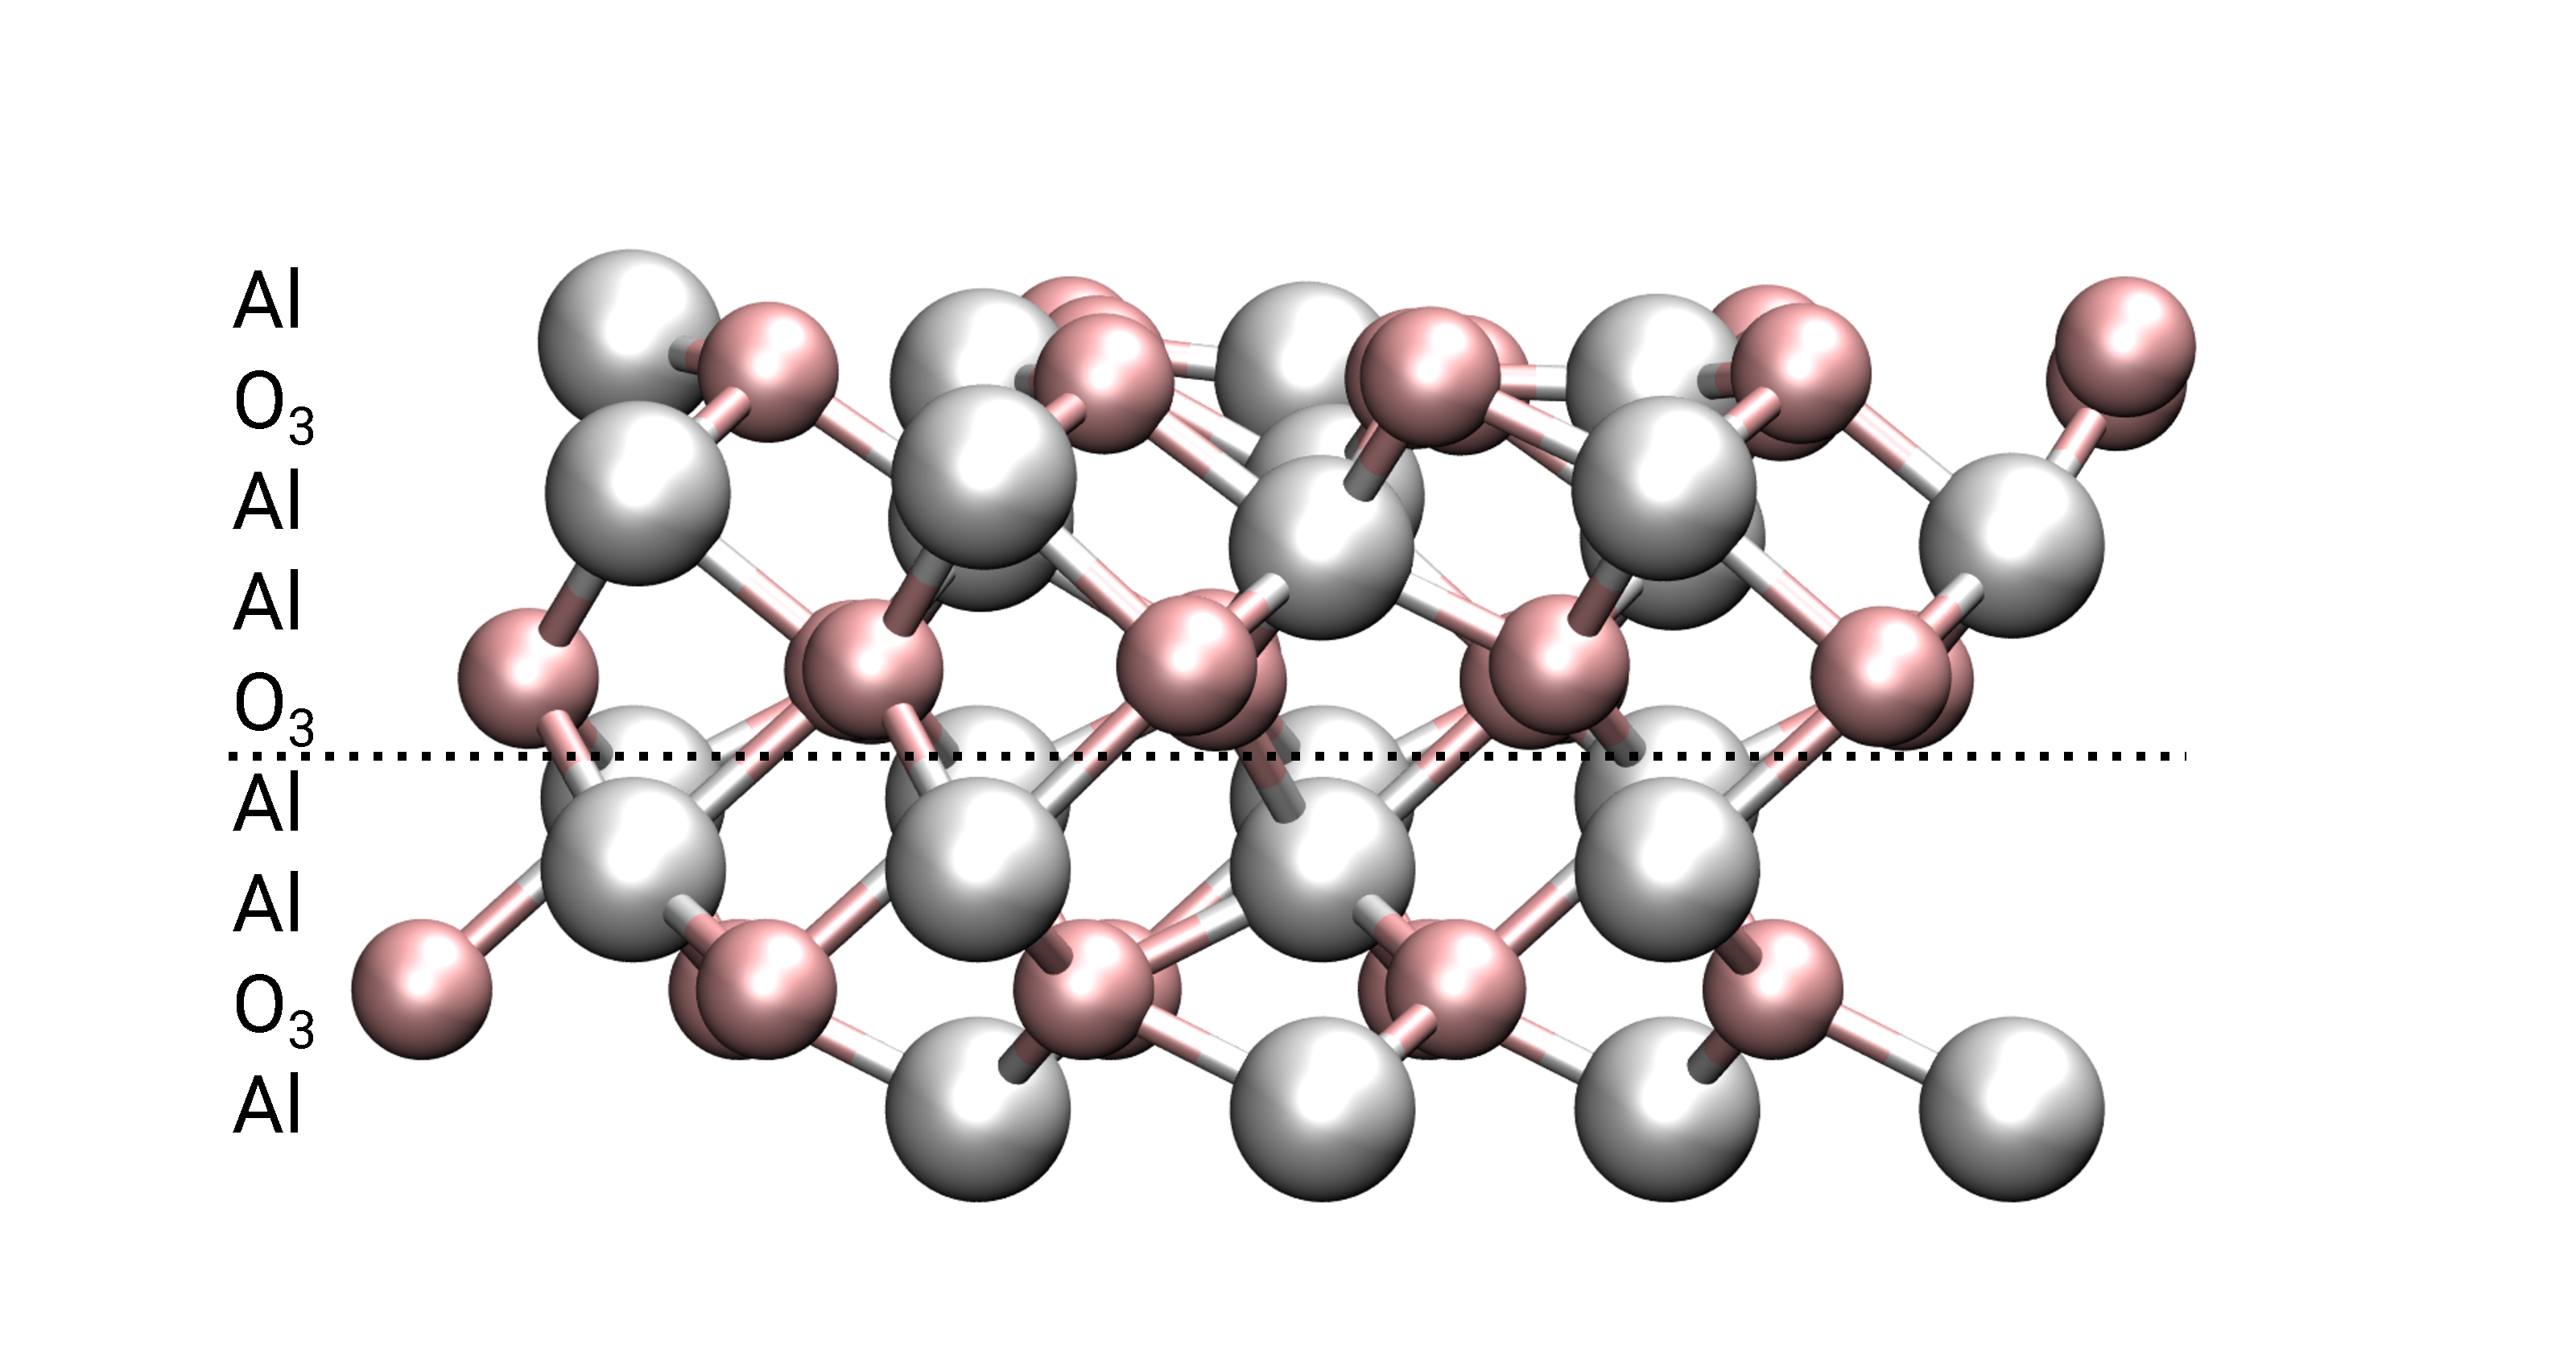
\includegraphics[width=1.\textwidth]{figures/surf_0K-side.pdf}
  \caption{Side view, atomic layers sequence Al-O$_3$-Al...}
  \end{figure}
  \end{columns}
 \hrule
 \begin{itemize}
  \item UHV $0\,$K geometry optimized structure
  \item Al terminated surface cut
  \item 4 CUS Al atoms, 12 threefold coordinated O atoms
  \item ($2\times 2$) supercell
 \end{itemize}
\end{frame}

\begin{frame}
 \frametitle{Adsorbed Species, Frequencies, and Reaction Path}
 \begin{itemize}
 \item Adsorption Energies $E_\textrm{ads}$ for most stable adsorbed species:\\~~~~~~~ mol ~~~~~~~~~~~~~~1-2 diss ~~~~~~~~~~~~1-4 diss
 \begin{figure}
  \centering
  \subfigure{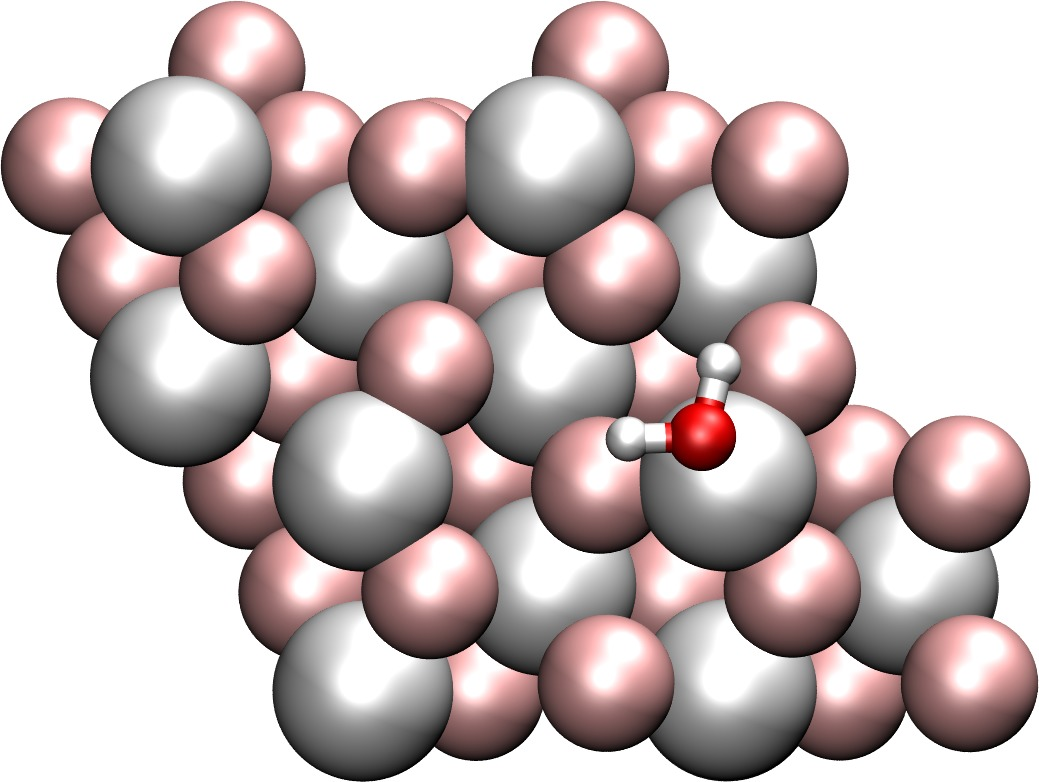
\includegraphics[width=0.25\textwidth]{figures/0001_mol_top.jpg}}
  \subfigure{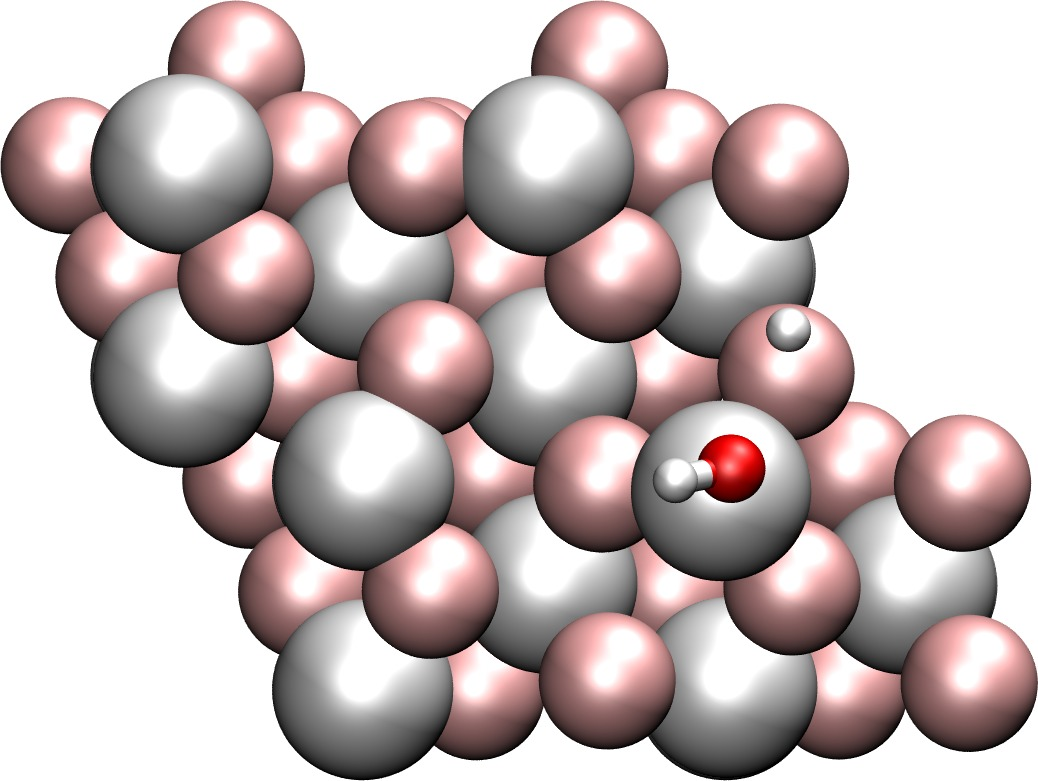
\includegraphics[width=0.25\textwidth]{figures/0001_1-2-diss_top.jpg}}
  \subfigure{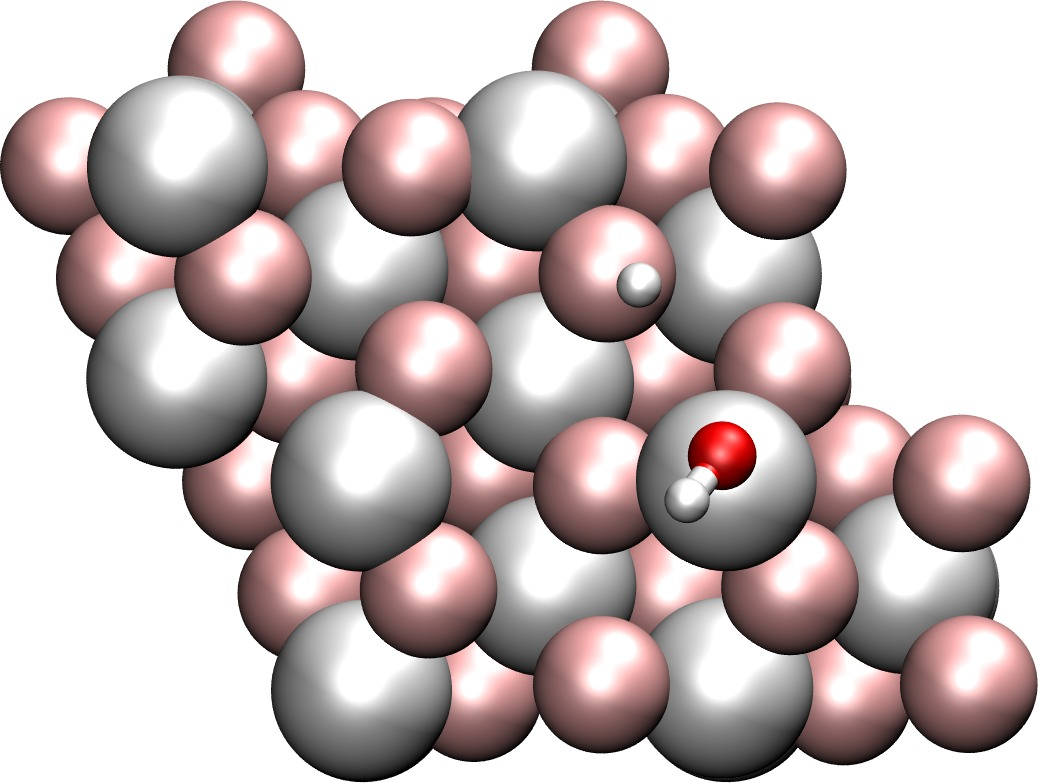
\includegraphics[width=0.25\textwidth]{figures/0001_1-4-diss_top.jpg}}
 \end{figure}
 \pause
 \item Vibrational frequencies for comparison with SFG spectroscopy
 \pause
 \item Diffusion reaction Df-H-4-2
 \begin{figure}
  \centering
  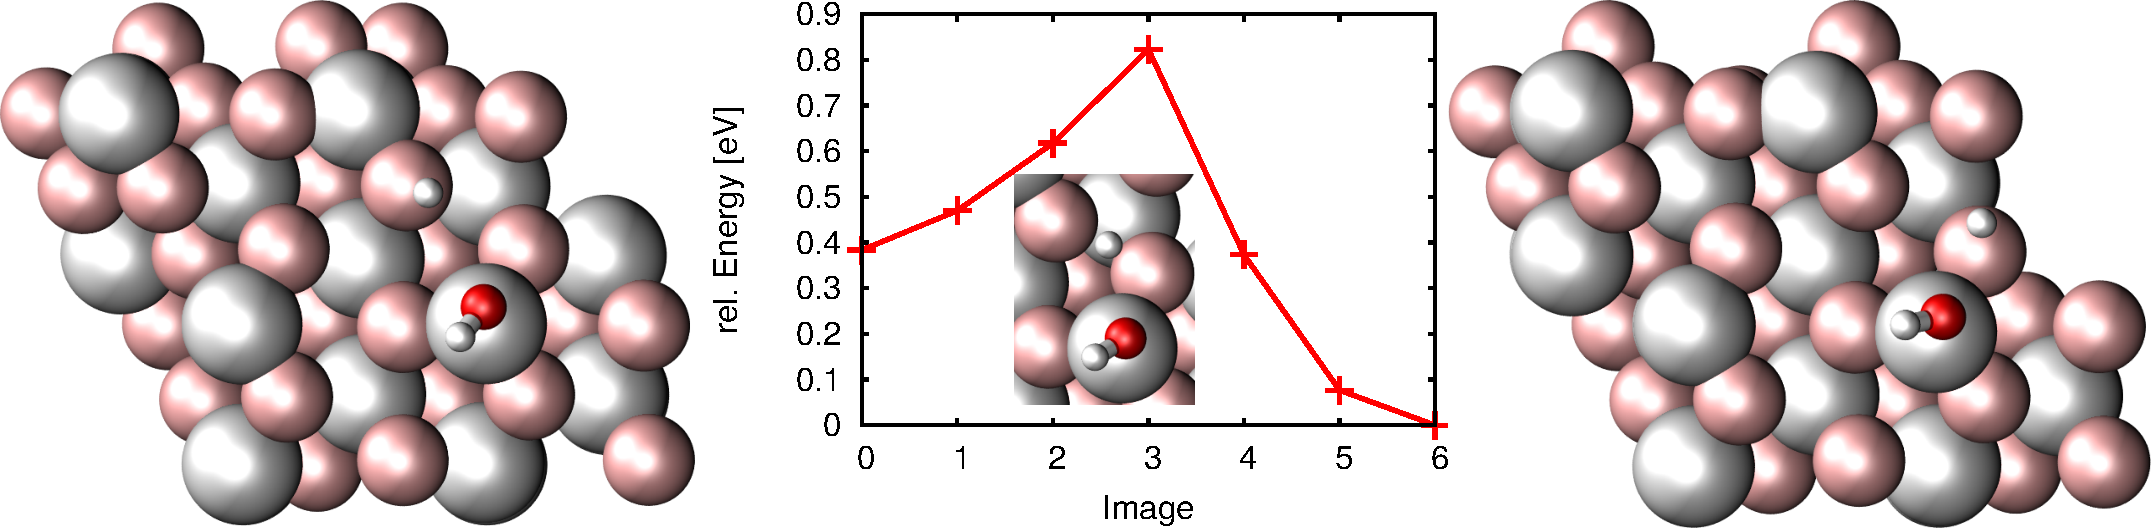
\includegraphics[width=.7\textwidth]{figures/df-h-4-2.pdf}
  \caption{1-4 to 1-2 hydrogen diffusion, NEB path with transition state}
 \end{figure}
 \end{itemize}
\end{frame}

\begin{frame}
 \frametitle{Adsorption Energies}
 \begin{table}[!h]
  \centering
   \caption{Adsorption energies $E_\textrm{ads}$ in eV of the molecular and two dissociated adsorption states of H$_2$O on the alumina(0001) surface, comparison of plane wave basis (PW) and atom orbital basis (AO).
   $E_{\textrm{ads}}=E_{\textrm{ads. species}}-(E_{\textrm{free water molecule}}+E_{\textrm{surface}})$}
  \begin{tabular}{ll|ccc}%c}
  \toprule
basis& method & mol & 1-2 diss & 1-4 diss\\\midrule
  \multirow{3}{1cm}{PW}&PW91 &{\color{orange}-1.25} &-1.59 &{\color{orange}-1.25} \\
  &PW91+D2&-1.40 &-1.81 &{\color{red}-1.45} \\
  &PBE+D2 & {\color{red}-1.31} & -1.69 & -1.21 \\
  %&PBE+D3 &-1.29&-1.63 &-1.30 \\
  \midrule \pause
  \multirow{4}{1cm}{AO}&PBE+D3 &{\color{red}-1.41} &-1.68 &-1.32 \\
  &B3LYP+D3 &{\color{red}-1.43} &-1.81 &-1.40 \\
  &HF &-1.14 &-1.67 &{\color{red}-1.19} \\
  &LMP2 &{\color{red}-1.34} & -1.69&-1.26\\
  %&LMP2 (basis 9) &-1.31 &-1.61 &-1.18 \\
  \bottomrule
  \end{tabular}
 \end{table}
\end{frame}

\begin{frame}
 \frametitle{Vibrational Frequencies of Dissociated Water Species}
 \begin{columns}
 \column{0.4\textwidth}
  \centering
  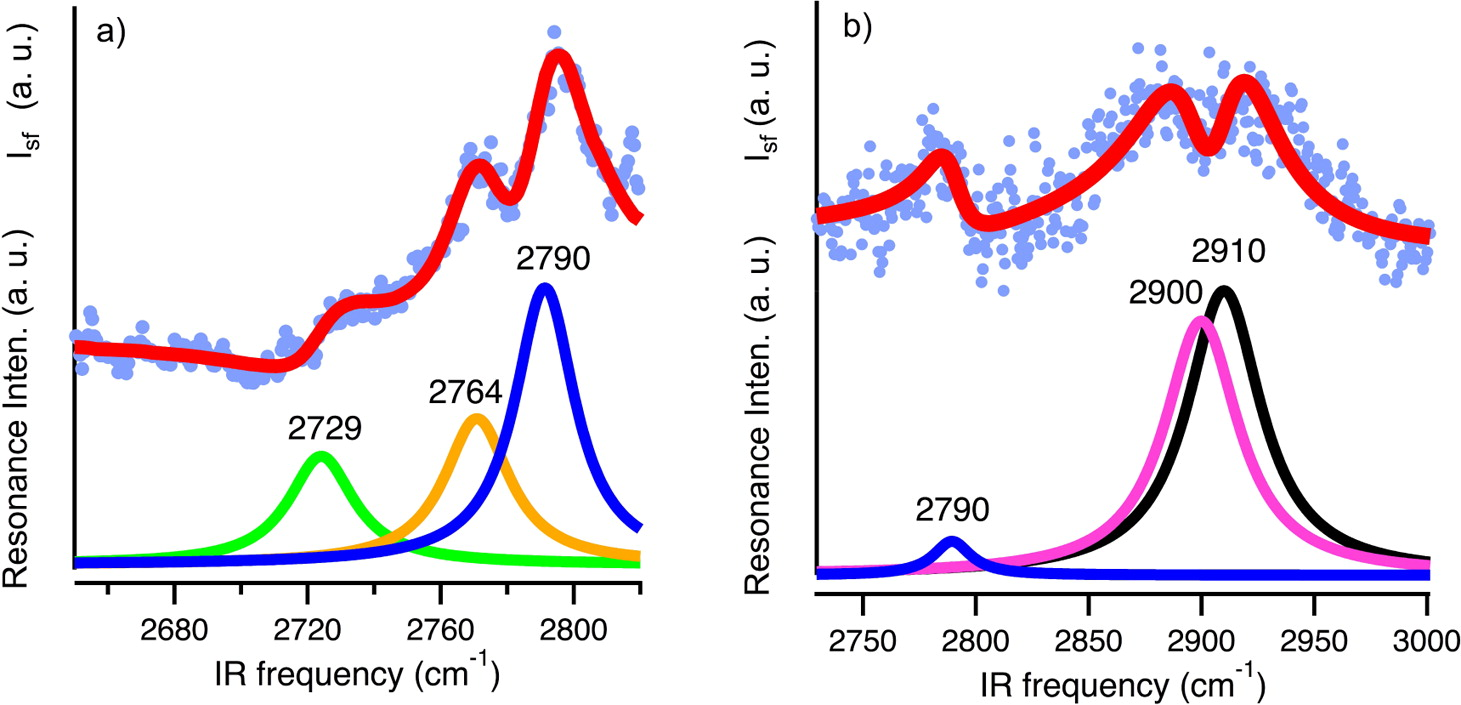
\includegraphics[width=1.1\textwidth]{figures/0001_OD_vib_exp.jpeg}\\
  \footnotesize{J. Phys. Chem. C \textbf{2014}, \textit{118}, 13623--13630.}
 \column{0.6\textwidth}
  \begin{table}[!h]
  \centering
  \begin{tabular}{l|cc}
  \toprule
 stretch &B3LYP+D3/AO & Exp.\\\midrule
 1-2 OD$_{surf}$&2697&2729\\
 1-4 OD$_{surf}$&2715&2764\\
%  1-4$^\prime$ OD$_{surf}$&2583&2790\\
 1-4 OD$_{ads}$&2873&2900\\
%  1-4$^\prime$ OD$_{ads}$&2697&2900\\
 1-2 OD$_{ads}$&2883&2910\\\bottomrule
  \end{tabular}
 \end{table}
 \end{columns}
 \vspace{-.5cm}
 \pause
  \begin{table}[!h]
  \centering
    \caption{Vibrational Frequencies $\Delta \tilde{\nu}$ of dissociated water species in cm$^{-1}$.}
    \vspace{-0.5cm}
  \begin{tabular}{c|cc|c|c}
  \toprule
& \multicolumn{2}{c}{AO} & PW & \\
 stretch &PBE+D3 & B3LYP+D3 & PBE+D2 & Exp.\\\midrule
 1-2 OD$_{\textrm{ads}}-$1-2 OD$_{surf}$& 212& 186& 181& 191 \\
 1-2 OD$_{\textrm{ads}}-$1-2 OD$_{ads}$ & 187& 168& 163& 146\\
 1-2 OD$_{\textrm{ads}}-$1-4 OD$_{surf}$& 13& 10& 15& 10\\\bottomrule
  \end{tabular}
 \end{table}
\end{frame} 

\begin{frame}
 \frametitle{Activation Barriers with Hybrid Functionals and LMP2}
 \begin{itemize}
  \item GGA functionals (here PBE) underestimate activation barriers $\rightarrow$ hybrid functional, perturbation theory
 \end{itemize}
 \centering
   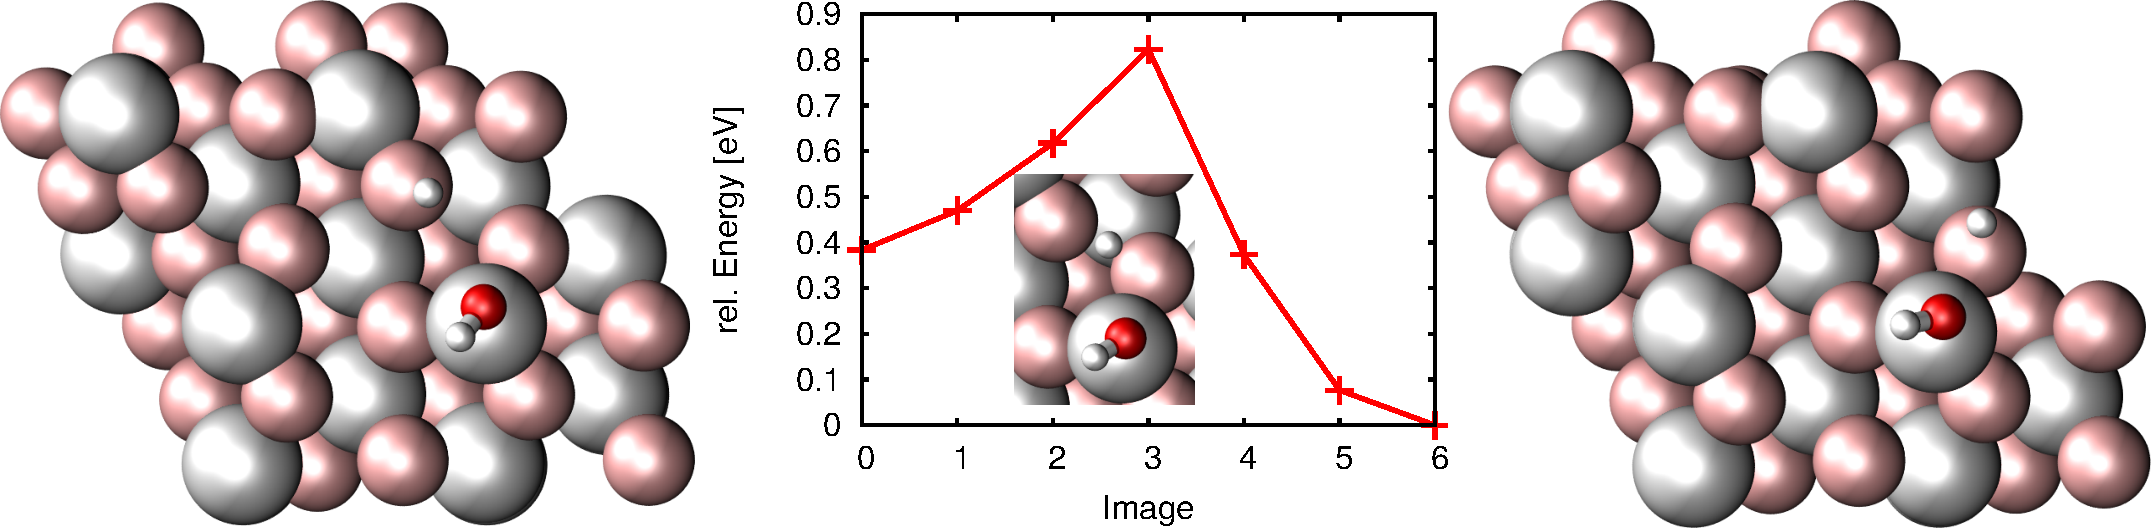
\includegraphics[width=.75\textwidth]{figures/df-h-4-2.pdf}
     \vspace{-.5cm}
     \pause
\begin{table}[!h]
  \centering
  \caption{$k(T)=\frac{k_BT}{h}e^{-\Delta G^\ddagger(T)/(k_BT)}$}
  \vspace{-.5cm}
  \begin{tabular}{l|cc|c}%|cc
  \toprule
    method& B3LYP+D3/AO&LMP2/AO &PBE+D2/PW\\\midrule
%     basis&AO-8&AO-9&PW\\\midrule
   $\Delta E^\ddagger$ [eV] &0.69 & 0.60&0.44\\
   $\Delta G^\ddagger$(300K) [eV]&0.58 & 0.49$^\ast$ &0.29\\
   $k$(300K) [s$^{-1}$]&$1.2\times 10^3$ & $3.7\times 10^{4\ast}$&$9.1\times 10^7$\\\bottomrule 
  \end{tabular}
\end{table}
$^\ast$ The contribution of the vibrations is estimated from B3LYP+D3, the corresponding rate is also affected by this approximation.
\end{frame} 

\begin{frame}
 \frametitle{Achievements}
 \begin{itemize}
  \item Recalculation of adsorption energies with atom centered orbital base
  \item Improvement of theoretical description of vibrational frequencies with respect to experimental values
  \item Improvement of activation barrier for diffusion reaction
 \end{itemize}
 \newline~\newline~\newline
 \centering
 \fbox{\parbox{\textwidth}{S. Heiden, D. Usvyat, P. Saalfrank, \textbf{2018}, \textit{in preparation}}}
\end{frame}

\section{Water@$\upalpha$-Al$_2$O$_3$(0001): Molecular Beam Scattering~~~~~~~~~~}
\begin{frame}
 \frametitle{Motivation: (0001) Molecular Beam Source}
Water probing at the surface: 
 \begin{itemize}
 \item MBS vs. pinhole dosing
 \item UHV, molecular beam onto surface vs. higher pressure
 \item non-equilibrium conditions vs. equilibrium situation
 \item {\color{red} enhanced dissociation probability with MBS}
 \newline~
 \pause \hrule
 \newline~
 \item model adsorption/dissociation process with \textit{ab initio} molecular dynamics simulations
 \item Employing different surface and beam models
\end{itemize}
\pause
\newline~\newline~
\fbox{\parbox{0.98\textwidth}{Heiden, S.; Wirth, J.; Campen, R. K.; Saalfrank, P., \textit{J. Phys. Chem. C} \textbf{2018}, \textit{122} (27), 15494--15504.}}
\end{frame}

\begin{frame}
 \frametitle{(0001) Surface and Beam Model}
 \begin{columns}
  \column{.5\textwidth}
  Surface Models
  \begin{itemize}
   \item Clean surface at $0$ and $300\,$K
   \item Preadsorbed surface at $0$ and $300\,$K
  \end{itemize} 
  \centering
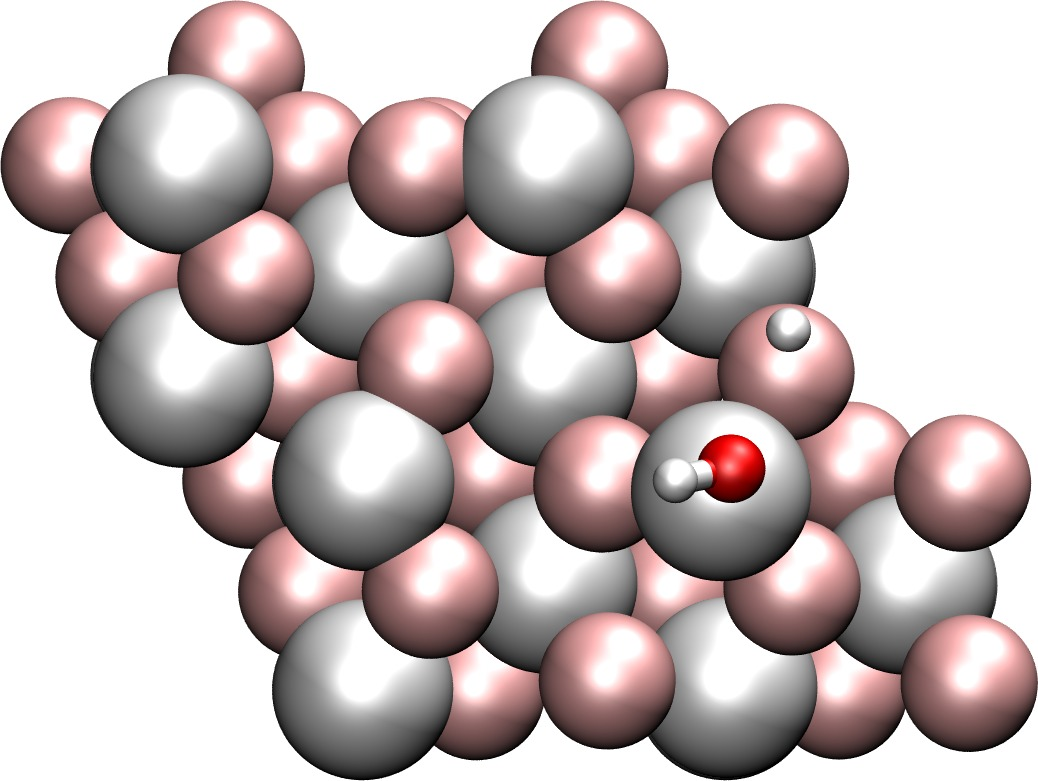
\includegraphics[width=1.\textwidth]{figures/0001_1-2-diss_top.jpg}
\newline
\pause
  \column{.5\textwidth}
  Beam Models
  \begin{itemize}
   \item Cold water molecule
   \item (D$_2$O)$_4$ cluster
   \item Rotationally/Vibrationally excited water
  \end{itemize}
   \centering
 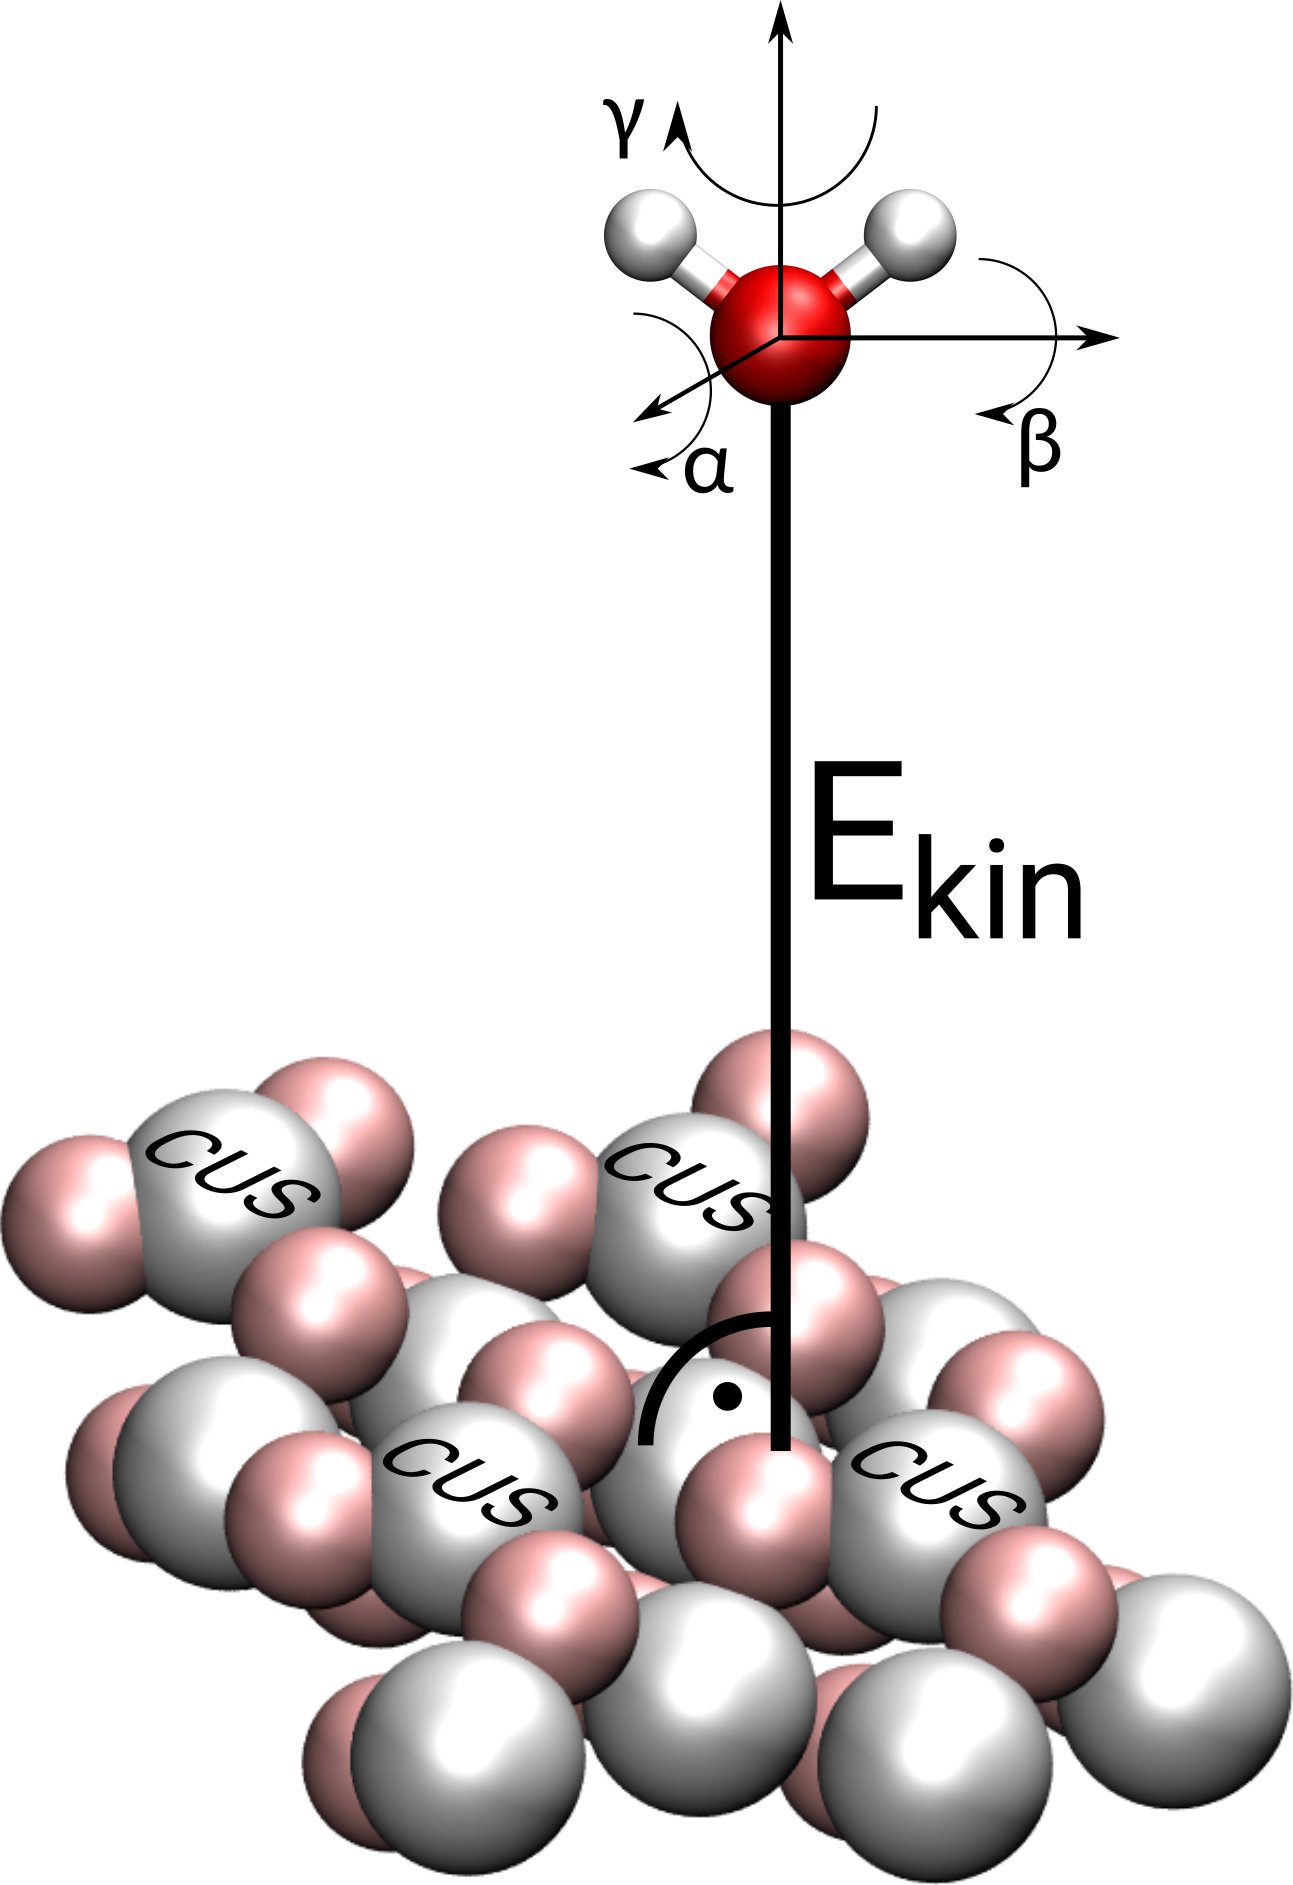
\includegraphics[width=0.5\textwidth]{figures/perspective+h2o_new.png}
\end{columns}
\end{frame}

\begin{frame}
 \frametitle{Adsorption and Dissociation Process}
 Example trajectories for molecular adsorption, dissociation
  \begin{figure}[h!]
  \centering
   \subfigure[molecular adsorption]{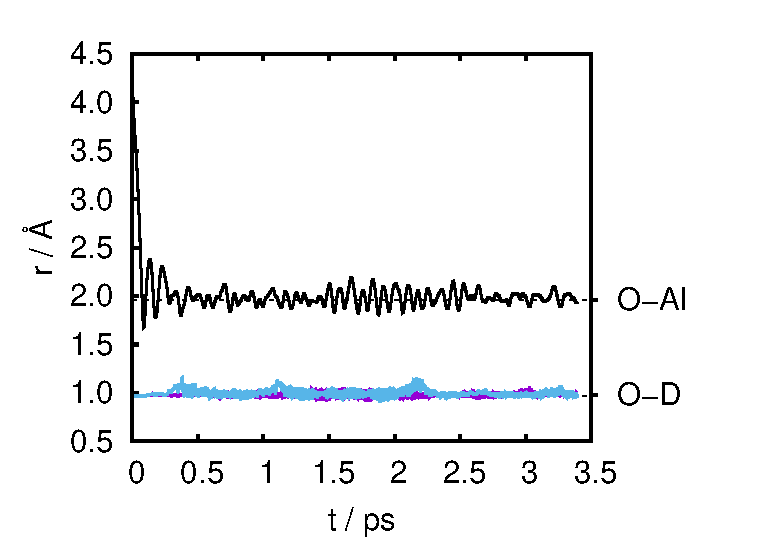
\includegraphics[width=0.35\textwidth]{figures/mol.eps}}
%    \quad
   \subfigure[1-2 dissociation]{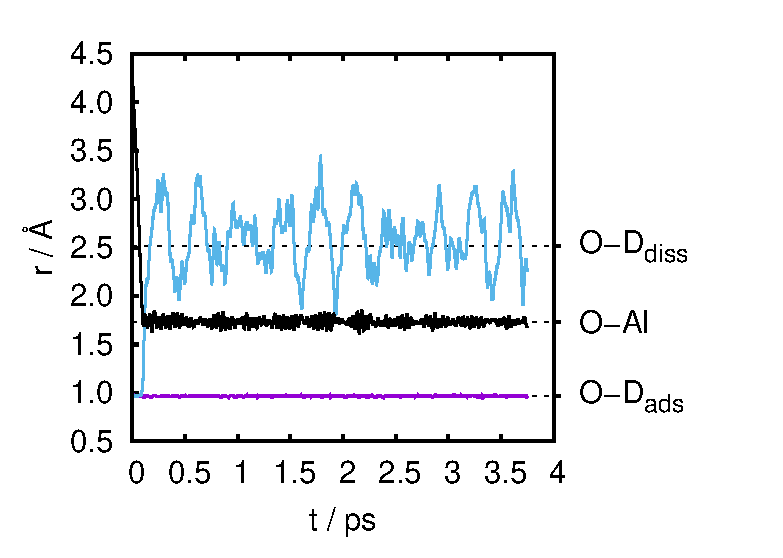
\includegraphics[width=0.35\textwidth]{figures/1-2.eps}}
 %    \quad\\
   \subfigure[1-4 dissociation]{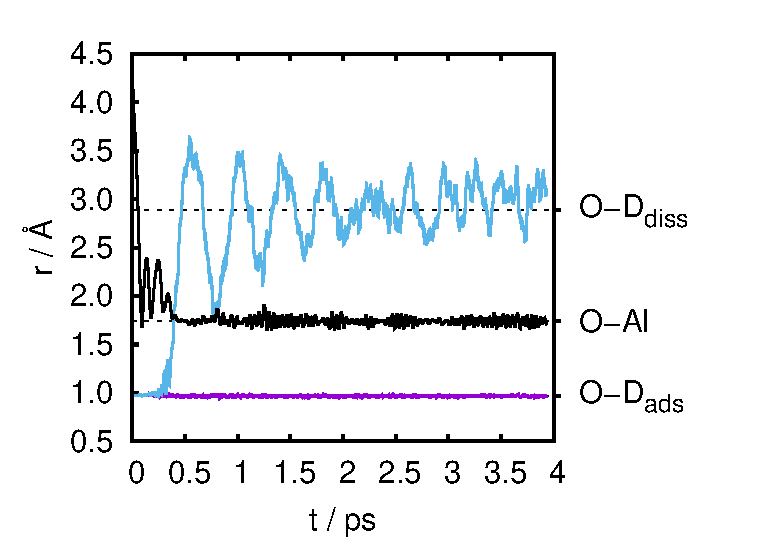
\includegraphics[width=0.35\textwidth]{figures/1-4.eps}}
%    \quad
   \subfigure[1-4$^\prime$ dissociation]{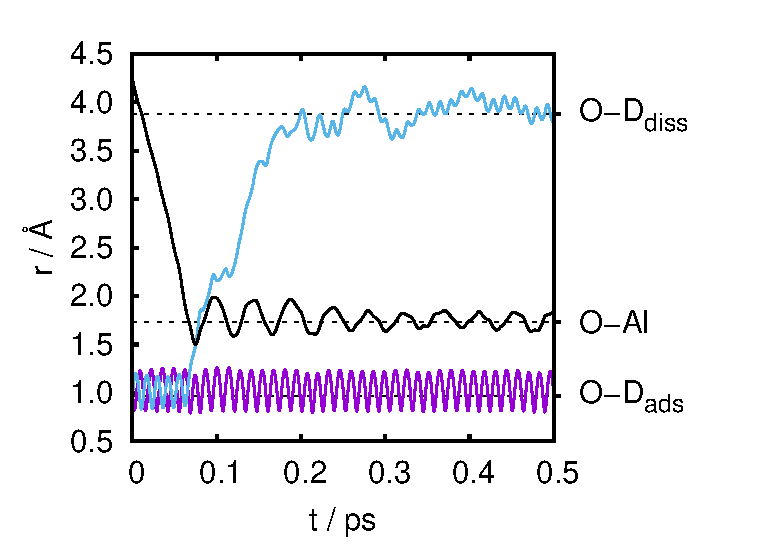
\includegraphics[width=0.35\textwidth]{figures/1-4d.eps}}
\end{figure}
   
\end{frame}


\begin{frame}
 \frametitle{Dissociation and Adsorption Probabilities}
 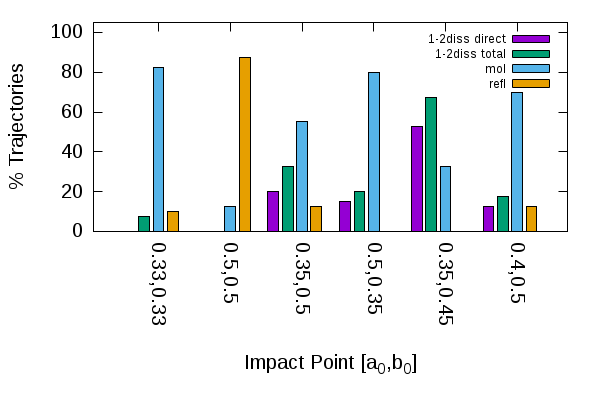
\includegraphics[width=0.45\textwidth]{figures/impactpoint.png}
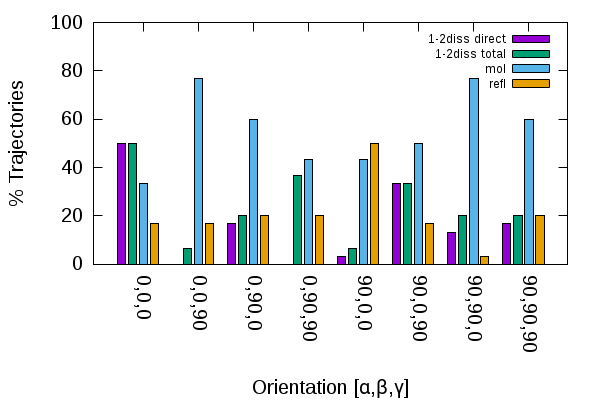
\includegraphics[width=0.45\textwidth]{figures/orientation.png}\hrule\pause
 \begin{columns}
  \column{0.5\textwidth}
  strongly dependent on
  \begin{itemize}
   \item impact site
   \item temperature effects
   \item precoverage
%    \item coverage
   \item vibrational excitation
  \end{itemize}
% \clearpage
  \column{0.5\textwidth}
  \newline less dependent on
  \begin{itemize}
   \item kinetic energy of the beam
   \item orientation of the molecule
  \end{itemize}
  \newline~\newline
  \clearpage
 \end{columns}
\\ 
\fbox{\parbox{0.98\textwidth}{Heiden, S.; Wirth, J.; Campen, R. K.; Saalfrank, P., \textit{J. Phys. Chem. C} \textbf{2018}, \textit{122} (27), 15494--15504.}}
\end{frame}


\section{Water@$\upalpha$-Al$_2$O$_3$(11\=20): Stability, Vibrations, and Reactivity}
\begin{frame}
 \frametitle{(11\=20) Surface}
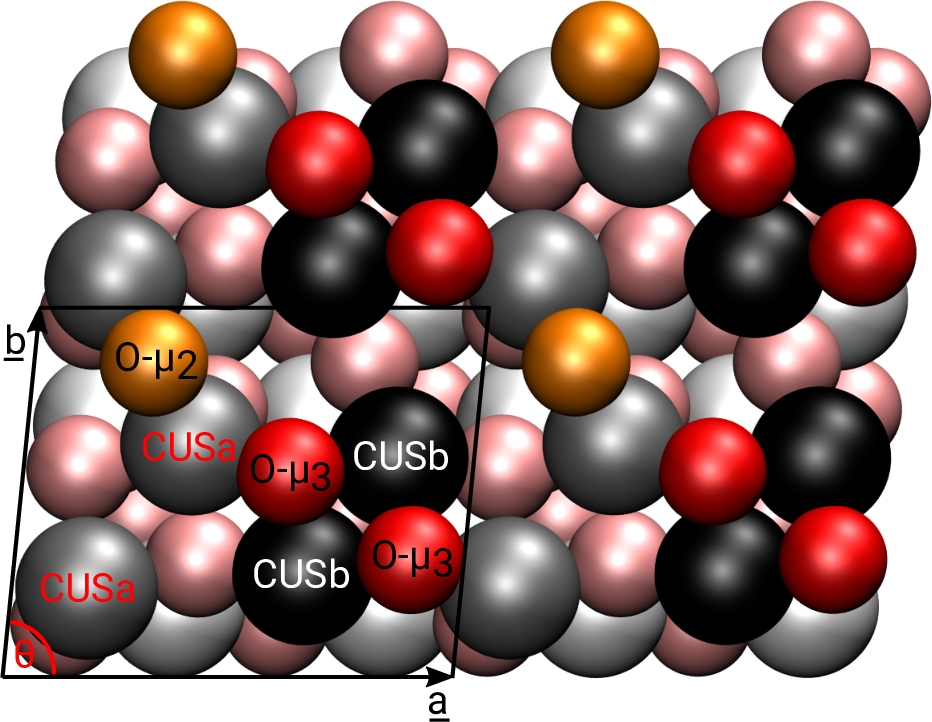
\includegraphics[width=0.4\textwidth]{figures/supercell_opt.png}
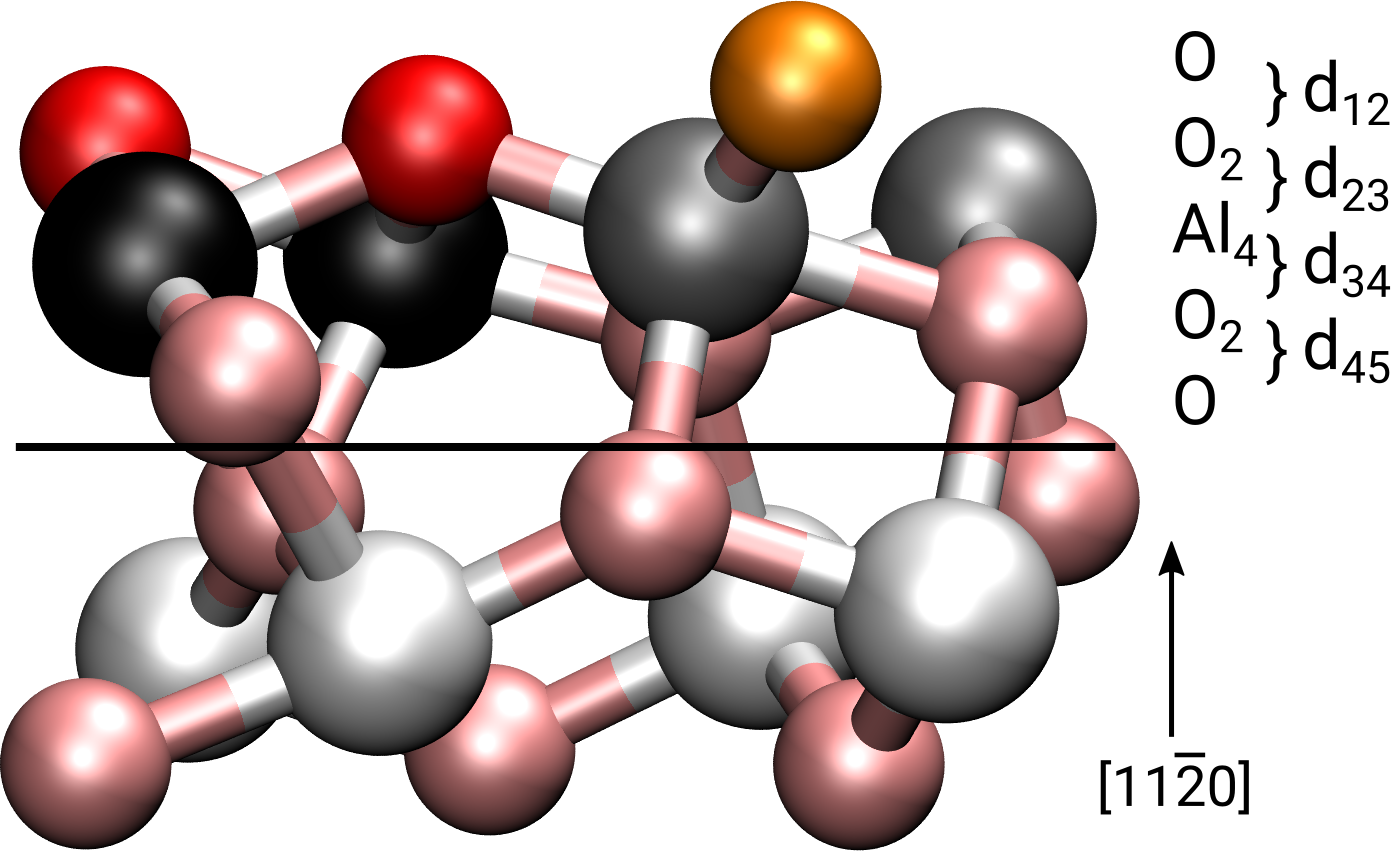
\includegraphics[width=0.4\textwidth]{figures/uc_opt.png}
(11\=20) surface, top view  ~ ~ ~~~~~~ (11\=20) side view
\newline
 \hrule
 \begin{itemize}
  \item UHV $0\,$K geometry optimized structure
  \item O-I terminated surface cut
  \item 8 CUSa and 8 CUSb Al atoms, 8 threefold coordinated and 4 twofold coordinated O atoms
  \item ($2\times 2$) supercell
 \end{itemize}
 \end{frame}

\begin{frame}
 \frametitle{Water Adsorption at the (11\=20) Surface}
 \centering
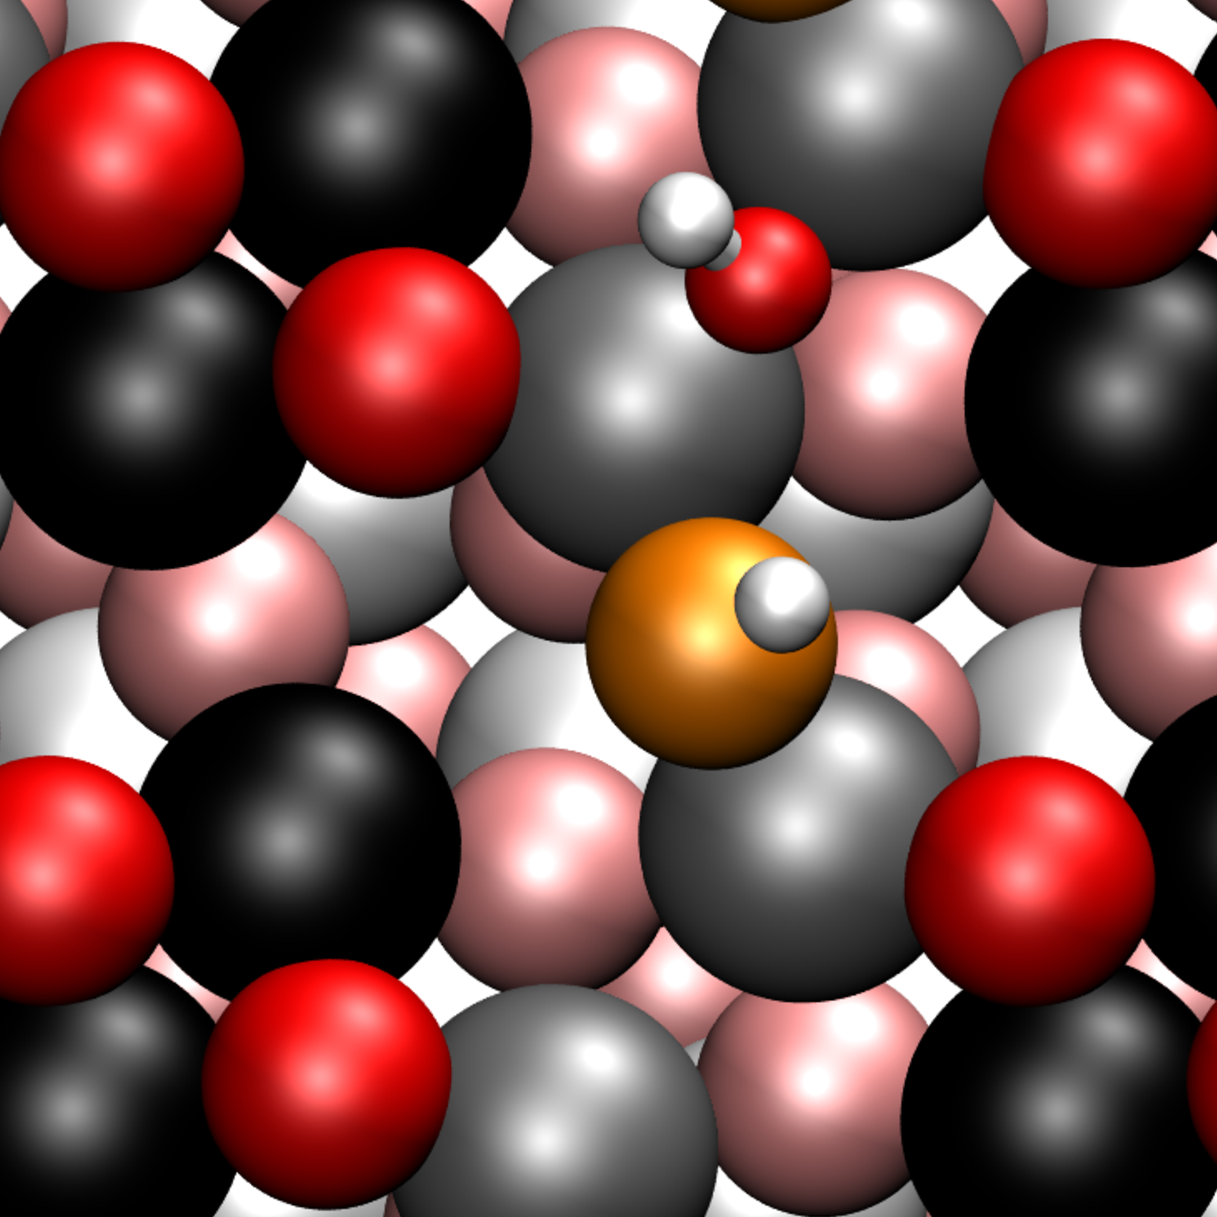
\includegraphics[width=0.25\textwidth]{figures/test-iCa2.pdf}~~~
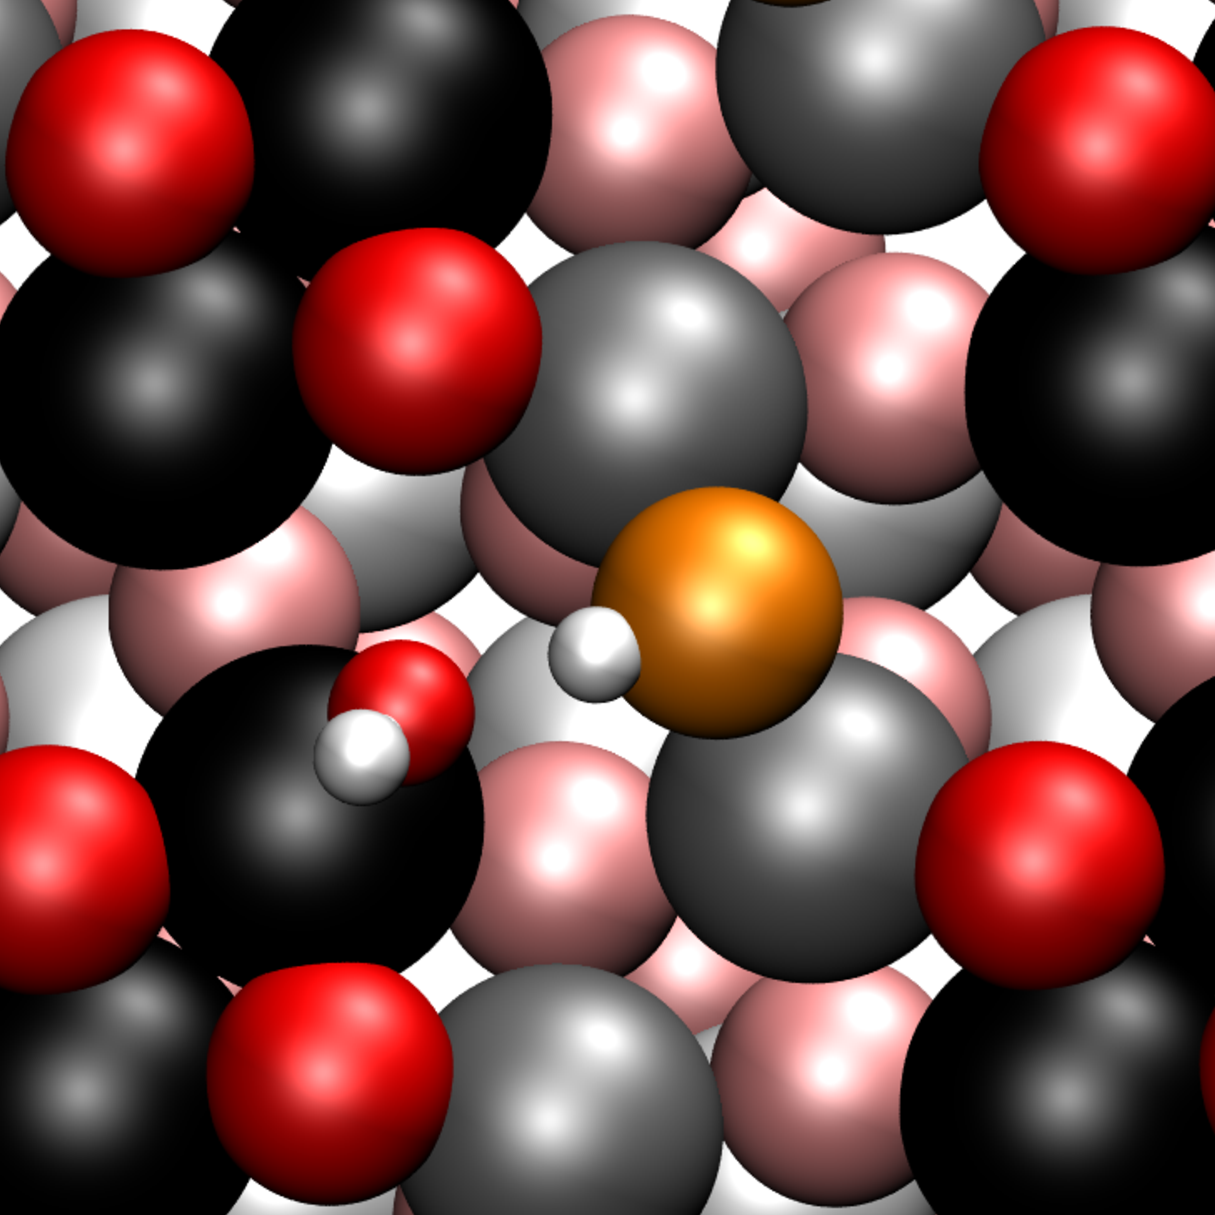
\includegraphics[width=0.25\textwidth]{figures/test-Cb2.pdf}~~~
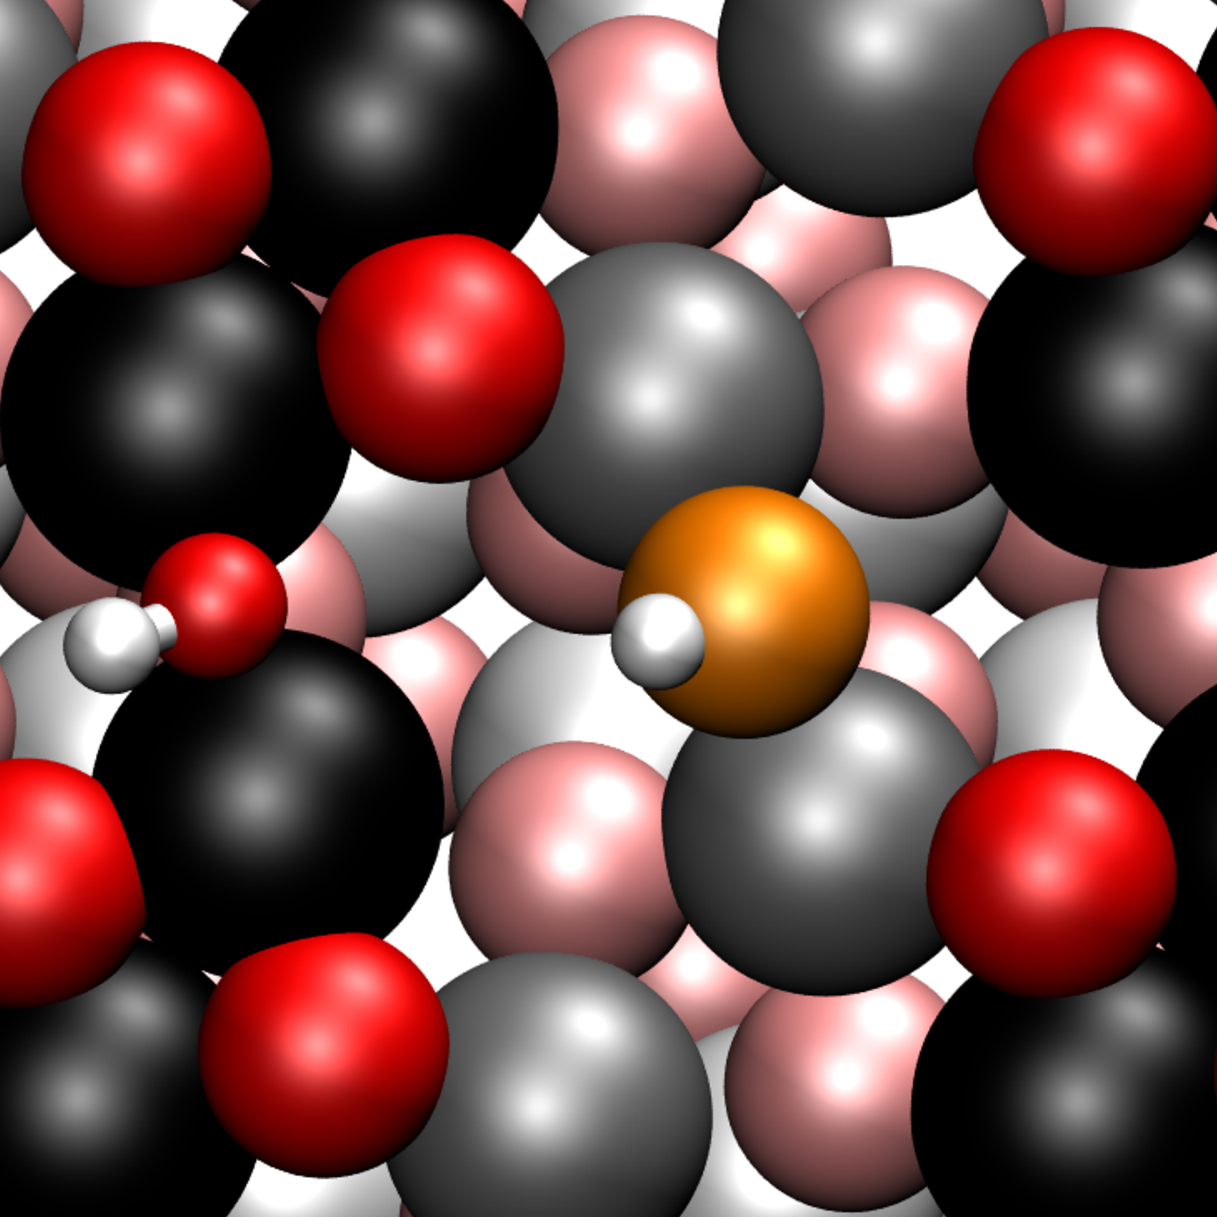
\includegraphics[width=0.25\textwidth]{figures/test-iCb2.pdf}~\newline
inter-CUSa$\parallel$O-$\mu_2$ ~~~~~CUSb$\parallel$O-$\mu_2$  ~~~~~inter-CUSb$\parallel$O-$\mu_2$~~~
\begin{table}[!ht]
  \centering
 \begin{tabular}{l|c}
  \toprule
   Adsorbed Species  & $E_\textrm{ads}$  \\\midrule
 CUSb          &   -1.78   \\\hline
 inter-CUSa$\parallel$O-$\mu_2$ & \textbf{-2.50}  \\
 inter-CUSa$\parallel$O-$\mu_3$ & -1.67  \\
 CUSb$\parallel$O-$\mu_2$ & \textbf{-2.28}  \\
 CUSb$\parallel$O-$\mu_3$ & -1.19  \\
 inter-CUSb$\parallel$O-$\mu_2$ & \textbf{-2.09} \\
 inter-CUSb$\parallel$O-$\mu_3$ & -1.89 \\\bottomrule
  \end{tabular}
  \label{tab:ads_1water}
\end{table}

\end{frame}

\begin{frame}
 \frametitle{Dissociation and Diffusion Reactions}
 Eyring equation: $k(T)=\frac{k_BT}{h}e^{-\Delta G^\ddagger/(k_BT)}$\newline~\newline
\begin{table*}
  \centering
  \begin{tabular}{ll|cc|c}
 \toprule
  \multicolumn{2}{c|}{\small{Reaction Type}}            & \small{$\Delta E^{\ddagger}$(eV)} & \small{$\Delta G^{\ddagger}_{\textrm{300\,K}}$(eV)} & \small{$k_{\textrm{300\,K}}$(s$^{-1}$)}  \\\midrule
\small{H$_2$O dissociation} &
   \small{\textit{D-I}}  &  \small{0.01} & \small{0.002} & \small{5.76$\times 10^{12}$} \\\midrule
 \small{OH diffusion} &
   \small{\textit{Df-OH-III}} &  \small{0.35} & \small{0.39} & \small{1.88$\times 10^6$}\\\midrule
%  & \small{Df-OH-IV}  & \small{1.07} & \small{1.10} & \small{2.41$\times 10^{-6}$} \\\midrule
\small{H diffusion} &
 \small{\textit{Df-H-V}}  & \small{1.65} & \small{1.49} & \small{4.90$\times 10^{-13}$} \\\bottomrule
% & \small{Df-H-VI} & \small{1.05} & \small{0.94} & \small{1.05$\times 10^{-3}$} \\\bottomrule
  \end{tabular}
  \label{tab:reaction-rates}
\end{table*}
\centering
\includegraphics<1>[width=0.8\textwidth]{figures/Diss_Cb-Cb2.pdf}\caption{H$_2$O dissociation}
\includegraphics<2>[width=.8\textwidth]{figures/Diff-OH_Cb2-iCb2.pdf}\caption{OH diffusion}
\includegraphics<3>[width=.8\textwidth]{figures/Diff-H_iCa2-iCa3p.pdf}\caption{H diffusion}
\end{frame}
 
\begin{frame}
 \frametitle{Vibrational Frequencies of OD Species}
 \begin{center}
  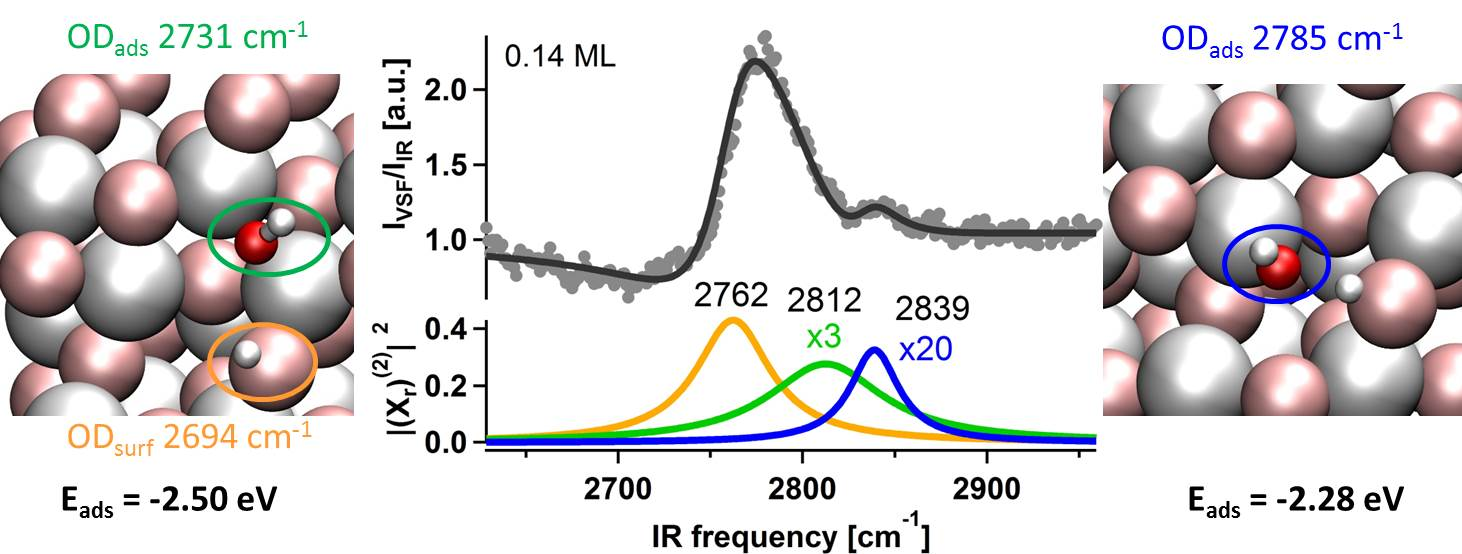
\includegraphics[width=0.75\textwidth]{figures/TOC_fig.jpg}
  \end{center}
\pause
\newline~
 \begin{tabular}{l|ccc|cc}
 \toprule
 Assigned species & $\tilde{\nu}_{\textrm{calc.}}$&$\Delta \tilde{\nu}_{\textrm{calc.}}$ &$\tilde{\nu}_{\textrm{exp.}}$ & $\Delta \tilde{\nu}_{\textrm{exp.}}$\\\midrule
  inter-CUSa$\parallel$O-$\mu_2$ OD$_\textrm{surf}$& 2694& & 2762& \\
  inter-CUSa$\parallel$O-$\mu_2$ OD$_\textrm{ads}$&2731 & 37 &2812 & 50\\
  CUSb$\parallel$O-$\mu_2$ OD$_\textrm{ads}$& 2785& 91 &2839 & 77 \\\bottomrule
  \end{tabular} 
\end{table*}  
\newline~\newline~\newline~
\fbox{\parbox{\textwidth}{Heiden, S.; Yue, Y.; Kirsch, H.; Wirth, J.; Saalfrank, P.; Campen, R. K., \textit{J. Phys. Chem. C} \textbf{2018}, \textit{122} (12), 6573--6584.}}
\end{frame} 

\begin{frame}
 \frametitle{Further Projects}
 \begin{columns}
 \column{0.55\textwidth}
 \begin{itemize}
  \item Lattice Al-O vibrations %\newline
 \end{itemize}
 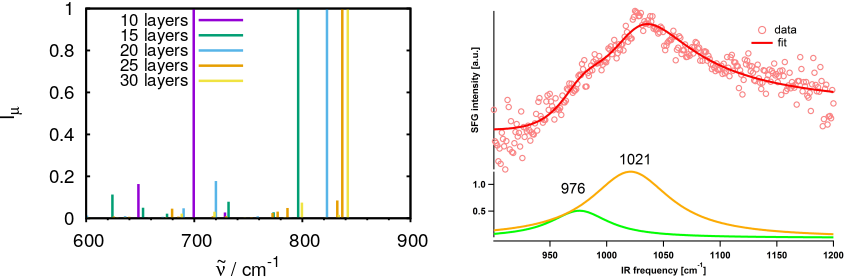
\includegraphics[width=0.9\textwidth]{figures/clean-surf-spectra.png}
 \begin{itemize}
 \item Higher water coverage
\end{itemize}
 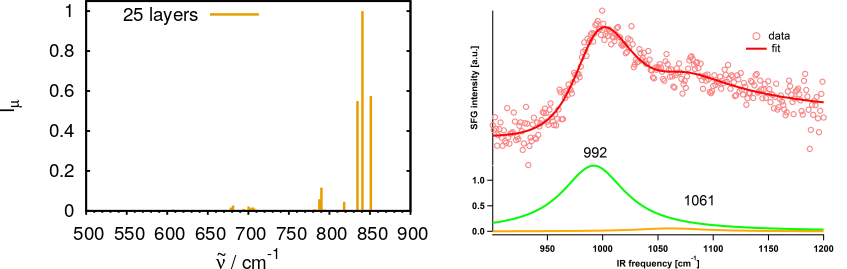
\includegraphics[width=0.9\textwidth]{figures/fully-cov-spectra.png}
 \column{0.225\textwidth}
 \begin{center}
 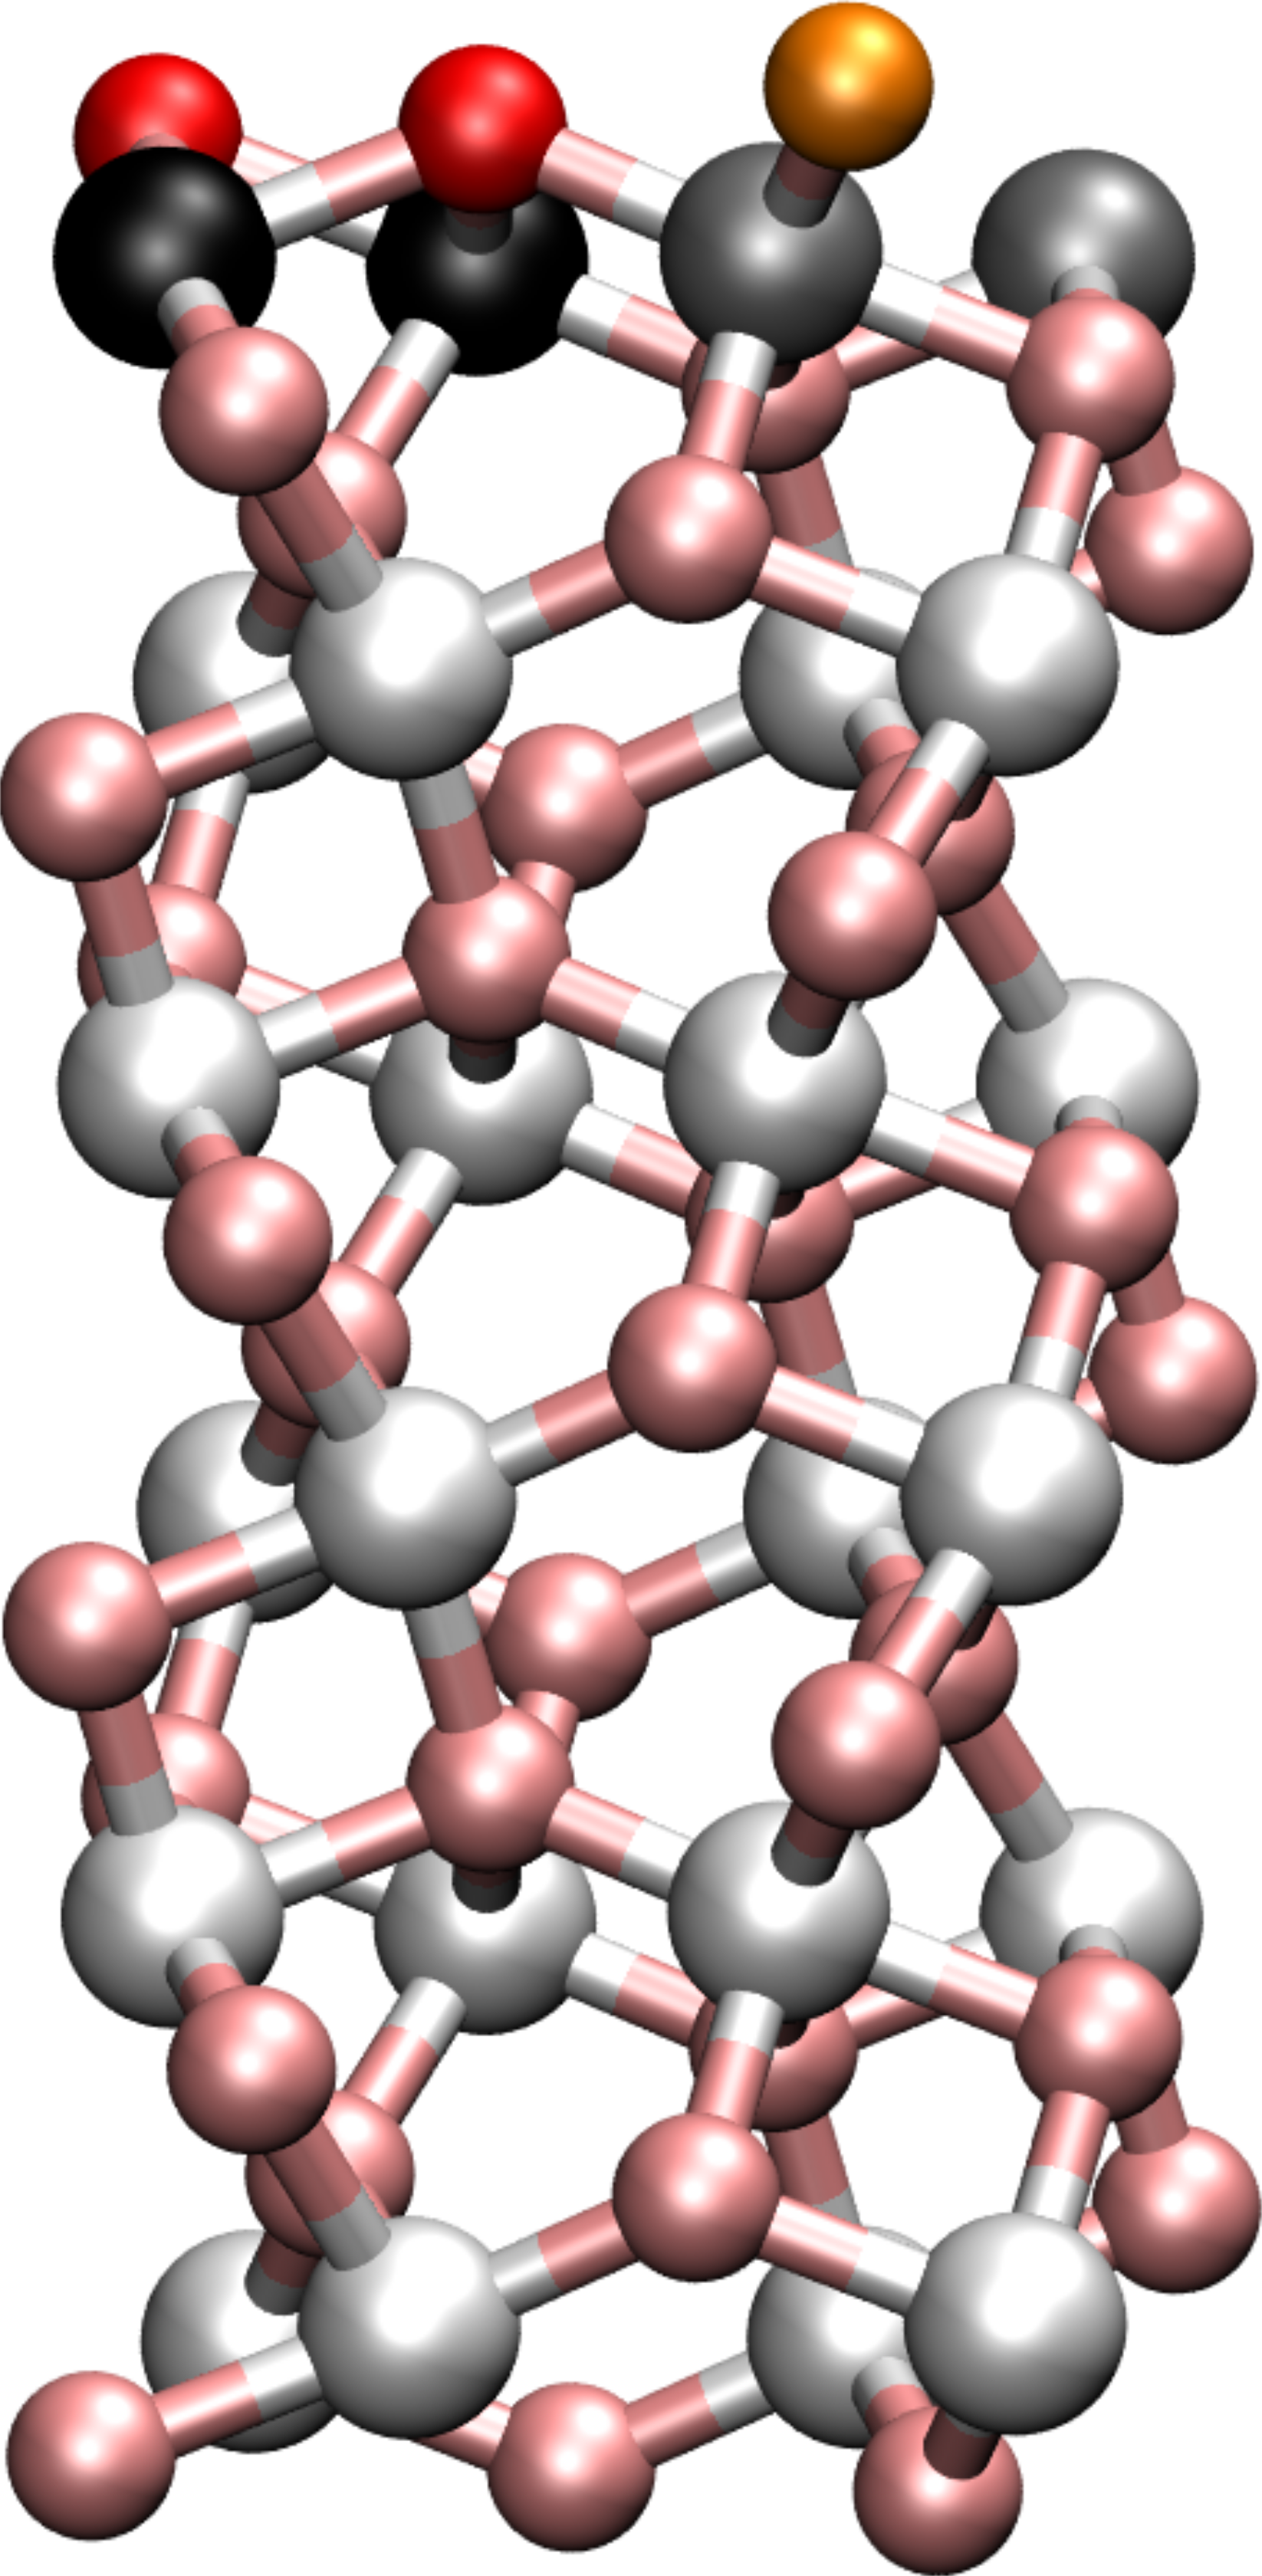
\includegraphics[width=.9\textwidth]{figures/30layer-model.png}~
 \end{center}
 \column{0.225\textwidth}
 \begin{center}
 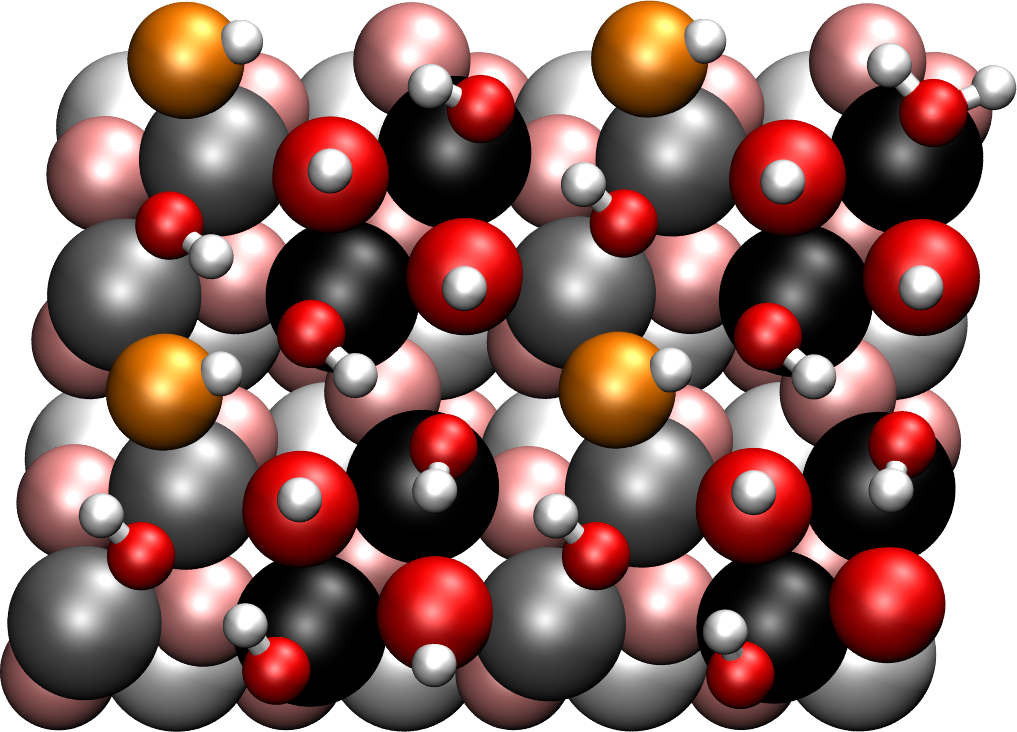
\includegraphics[width=.9\textwidth]{figures/O-I-fully.png}
 \end{center}
 \end{columns}
 \newline~\newline~\newline
\fbox{\parbox{\textwidth}{Yue, Y.; Heiden, S.; Kirsch, H.; Wirth, J.; Campen, R. K.; Saalfrank, P., in preparation}}
\end{frame}


\section*{}
\begin{frame}
 \frametitle{Summary and Outlook}
 {\color{blue}(0001) Surface}
\begin{itemize}
 \item Recalculation of E$_{\textrm{ads}}$ 
 \item Vibrational frequency calculation improved w.r.t. experiment
 \item Activation and rate constant improvement
\end{itemize}
 \pause\hrule
\begin{itemize}
 \item MBS scattering
 \item Understand enhanced dissociation
 \item Mechanism of water adsorption/dissociation
\end{itemize}
 \pause\hrule
 {\color{blue}(11\=20) Surface}
\begin{itemize}
 \item Structure search and adsorption energies
 \item Vibrational frequencies of water and surface species
 \item Analyses of surface reactions
\end{itemize}
 \end{frame}

\begin{frame}
 \frametitle{Acknowledgment}
 \begin{columns}
    \column{0.8\textwidth}
 \begin{itemize}
  \item Prof. Dr. Peter Saalfrank
  \item Prof. Dr. Beate Paulus (FU Berlin)
  \item PD Dr. Tillmann Klamroth
  \item Dr. R. K. Campen \& Yanhua Yue (FHI Berlin)
  \item Dr. Denis Usvyat (HU Berlin)
  \item AG TC, especially: G. Melani, Dr. J. Wirth, Dr. R. W\l{}odarczyk, Spa\ss{}raum 2
 \end{itemize}
 \column{0.2\textwidth}
 \centering

\includegraphics[width=1cm]{figures/crc1109.png}
\\

\includegraphics[width=2cm]{figures/hlrn_logo.png}
\end{columns}
\centering
\includegraphics[width=8cm]{figures/ag-wise1718.png}

\end{frame}

 \end{document}
